% Options for packages loaded elsewhere
\PassOptionsToPackage{unicode}{hyperref}
\PassOptionsToPackage{hyphens}{url}
%
\documentclass[
]{article}
\usepackage{lmodern}
\usepackage{amssymb,amsmath}
\usepackage{ifxetex,ifluatex}
\ifnum 0\ifxetex 1\fi\ifluatex 1\fi=0 % if pdftex
  \usepackage[T1]{fontenc}
  \usepackage[utf8]{inputenc}
  \usepackage{textcomp} % provide euro and other symbols
\else % if luatex or xetex
  \usepackage{unicode-math}
  \defaultfontfeatures{Scale=MatchLowercase}
  \defaultfontfeatures[\rmfamily]{Ligatures=TeX,Scale=1}
\fi
% Use upquote if available, for straight quotes in verbatim environments
\IfFileExists{upquote.sty}{\usepackage{upquote}}{}
\IfFileExists{microtype.sty}{% use microtype if available
  \usepackage[]{microtype}
  \UseMicrotypeSet[protrusion]{basicmath} % disable protrusion for tt fonts
}{}
\makeatletter
\@ifundefined{KOMAClassName}{% if non-KOMA class
  \IfFileExists{parskip.sty}{%
    \usepackage{parskip}
  }{% else
    \setlength{\parindent}{0pt}
    \setlength{\parskip}{6pt plus 2pt minus 1pt}}
}{% if KOMA class
  \KOMAoptions{parskip=half}}
\makeatother
\usepackage{xcolor}
\IfFileExists{xurl.sty}{\usepackage{xurl}}{} % add URL line breaks if available
\IfFileExists{bookmark.sty}{\usepackage{bookmark}}{\usepackage{hyperref}}
\hypersetup{
  hidelinks,
  pdfcreator={LaTeX via pandoc}}
\urlstyle{same} % disable monospaced font for URLs
\usepackage[margin=1in]{geometry}
\usepackage{graphicx}
\makeatletter
\def\maxwidth{\ifdim\Gin@nat@width>\linewidth\linewidth\else\Gin@nat@width\fi}
\def\maxheight{\ifdim\Gin@nat@height>\textheight\textheight\else\Gin@nat@height\fi}
\makeatother
% Scale images if necessary, so that they will not overflow the page
% margins by default, and it is still possible to overwrite the defaults
% using explicit options in \includegraphics[width, height, ...]{}
\setkeys{Gin}{width=\maxwidth,height=\maxheight,keepaspectratio}
% Set default figure placement to htbp
\makeatletter
\def\fps@figure{htbp}
\makeatother
\setlength{\emergencystretch}{3em} % prevent overfull lines
\providecommand{\tightlist}{%
  \setlength{\itemsep}{0pt}\setlength{\parskip}{0pt}}
\setcounter{secnumdepth}{-\maxdimen} % remove section numbering
\ifluatex
  \usepackage{selnolig}  % disable illegal ligatures
\fi
\newlength{\cslhangindent}
\setlength{\cslhangindent}{1.5em}
\newenvironment{cslreferences}%
  {\setlength{\parindent}{0pt}%
  \everypar{\setlength{\hangindent}{\cslhangindent}}\ignorespaces}%
  {\par}

\author{}
\date{\vspace{-2.5em}}

\begin{document}

\raggedright

\textbf{Title:} Using tree-ring records to simultaneously characterize
the influence of tree size and climate drivers on annual growth

\textbf{Authors:}

\href{0000-0001-8461-9713}{Kristina J.
Anderson-Teixeira\textsuperscript{1,2}*}, Valentine
Herrmann\textsuperscript{1}, Christy Rollinson\textsuperscript{3},
Bianca Gonzalez\textsuperscript{1}, Erika B.
Gonzalez-Akre\textsuperscript{1}, Neil Pederson\textsuperscript{4},
Camille Piponiot\textsuperscript{1,2}, Ross Alexander, Craig D. Allen,
Raquel Alfaro-Sánchez\textsuperscript{wl}, Tala Awada, Jennifer
Baltzer\textsuperscript{wl}, Patrick Baker, Sarayudh Bunyavejchewin,
Paolo Cherubini, Justin Cooper, Stuart Davies\textsuperscript{2}, Ryan
Helcoski\textsuperscript{1}, \href{0000-0003-1780-6310}{Jakub
Kašpar\textsuperscript{cz}}, James Lutz, Ellis Q. Margolis, Justin
Maxwell\textsuperscript{jm}, Sean McMahon\textsuperscript{2}, Sabrina
Russo, \href{0000-0002-7722-8797}{Pavel Šamonil\textsuperscript{cz}},
Anastasia Sniderhan\textsuperscript{wl}, Alan J.
Tepley\textsuperscript{1,at}, \href{0000-0002-6070-5956}{Ivana
Vašíčková\textsuperscript{cz}}, Mart Vlam, Peter Zuidema

\textbf{Author Affiliations:}

\begin{enumerate}
\def\labelenumi{\arabic{enumi}.}
\item
  Conservation Ecology Center; Smithsonian Conservation Biology
  Institute; Front Royal, VA 22630, USA
\item
  Center for Tropical Forest Science-Forest Global Earth Observatory;
  Smithsonian Tropical Research Institute; Panama, Republic of Panama
\item
  The Morton Arboretum, Lisle, Illinois, USA
\item
  Harvard Forest, Petersham, MA 01366, USA
\end{enumerate}

wl. Biology Department, Wilfrid Laurier University, 75 University Ave W,
Waterloo, ON, N2L 3C5

at. Canadian Forest Service, Northern Forestry Centre, Edmonton,
Alberta, Canada

cz. Department of Forest Ecology, The Silva Tarouca Research Institute
for Landscape and Ornamental Gardening, Lidická 25/27, 602 00 Brno,
Czech Republic

jm. Department of Geography, Indiana University, Bloomington, Indiana,
USA

*corresponding author:
\href{mailto:teixeirak@si.edu}{\nolinkurl{teixeirak@si.edu}}; +1 540 635
6546

\textbf{Running headline:} {[}45 chars{]}

\newpage

\hypertarget{abstract}{%
\section{Abstract}\label{abstract}}

\begin{enumerate}
\def\labelenumi{\arabic{enumi}.}
\item
  Tree rings provide a valuable long-term record for understanding how
  climate shapes forest productivity. However, traditional analysis
  methods aggregate growth records of multiple trees into residual
  chronologies, and therefore cannot simultaneously account for the
  effects of tree size and climate. This has limited the potential to
  use tree-rings to understand forest productivity and its climate
  sensitivity.
\item
  Here, we develop a new method to simultaneously model non-linear
  effects of objectively determined principle climate drivers and
  reconstructed tree diameter (\(DBH\)). Specifically, we first identify
  the most important climate drivers and their appropriate time window
  of influence using the \emph{climwin} R package. We then include these
  in generalized least squares models to model tree growth while
  accounting for the temporal autocorrelation inherent to each
  individual tree's growth. We apply this method to tree-ring data from
  1822 trees representing 39 species at ten globally distributed sites
  spanning a wide range of forest types.
\item
  Our analysis identified similar climate drivers operating over similar
  time windows to those obtained via traditional methods, but revealed
  that non-linear responses to climate variables were common. Growth
  rates--expressed as ring widths, basal area increments, or biomass
  increments--varied non-linearly with \(DBH\). The relative importance
  of \(DBH\) versus climate varied across sites, and interactions
  between \(DBH\) and climate were prevalent (\emph{\textasciitilde50\%}
  of cases tested).
\item
  Our method provides a rigorous analytical framework for objectively
  identifying the most important climate drivers of tree growth and
  combining them with \(DBH\) in nonlinear models. The need for such an
  approach is highlighted by our findings that nonlinear growth
  responses to climate variables are common, that growth rates vary
  nonlinearly with \(DBH\), and that significant \(DBH\) - climate
  interactions are common. These findings imply that \(DBH\) should be
  accounted for in analyses seeking to quantify the impacts of climate
  and other environmental drivers on tree growth. By providing a
  framework for such analyses, our approach opens the door for using
  tree-rings to improve our understanding of forest responses to climate
  change.
\end{enumerate}

\textbf{Keywords}: climate sensitivity; diameter; environmental change;
Forest Global Earth Observatory (ForestGEO); generalized least squares;
nonlinear; tree-ring

\newpage

\hypertarget{introduction}{%
\section{Introduction}\label{introduction}}

\textbf{Tree rings provide a long-term record of annual growth
increments that is invaluable for understanding forests in an era of
global change.} Spanning time scales of decades to centuries or even
millennia, they provide by far the most robust method for
characterization of the interannual climate sensitivity of tree growth
(Fritts, 1976) and how it is changing (e.g., Sniderhan \& Baltzer, 2016;
Maxwell, Harley, \& Robeson, 2016). Combined with forest censuses, they
can be used to estimate forest woody productivity (\(ANPP_{woody}\);
Graumlich, Brubaker, \& Grier, 1989; Teets, Fraver, et al., 2018) and
its climate sensitivity (Klesse et al., 2018; Teets et al., 2018;
Helcoski et al., 2019). This information is critical to predicting
forest responses to climate change, and thereby reducing the enormous
uncertainty surrounding future contributions of Earth's forests to the
global carbon cycle (Friedlingstein et al., 2006). Yet,
dendrochronological methods have been optimized to detect climate
signals rather than to predict forest productivity and its climate
sensitivity (Klesse et al., 2018). As a result, prevailing approaches
hold a number of limitations for using tree-rings to address pressing
questions concerning forest productivity in the current era of rapid
environmental change.

\textbf{To predict annual tree growth or forest productivity based on
climate, a necessary first step is identification of the most important
climate variables, the time frames over which they have the strongest
influence over annual growth, and their additive or interactive
effects.} Traditional dendrochronological methods identify climate
signals by examining month-by-month correlations of ring-width index
chronologies to select climate variables--most commonly temperature,
precipitation, or a moisture index (PDSI or SPEI)--over the current year
and, typically, previous year (e.g., Fritts, 1976; Zang \& Biondi,
2015). While appropriate for identifying the strongest correlation
between tree growth and an individual climate variable for purposes such
as historical climate reconstructions (e.g., Pederson et al., 2013;
Maxwell \& Harley, 2017) and for describing how each month's climate
affects tree growth or productivity (e.g., Helcoski et al., 2019), this
approach falls short of objectively identifying the most important
climate drivers and their time windows of influence, which is needed for
multivariate models of annual tree growth and forest productivity (e.g.,
Teets et al., 2018). Further, tree-ring studies generally do not
consider additive or interactive effects of climate variables on annual
growth (DENDRO\_REFS; but see Foster, Finley, D'Amato, Bradford, \&
Banerjee, 2016). Such effects are expected based on observations that
temperature and moisture jointly shape photosynthesis (REFS), tree
growth (Beedlow, Lee, Tingey, Waschmann, \& Burdick, 2013; Foster et
al., 2016), and forest productivity (e.g., Alexander, Rollinson, Babst,
Trouet, \& Moore, 2018; Banbury Morgan et al., n.d.). Thus, to model
tree growth responses to climate, we need an objective approach to
systematically evaluate numerous potential climate variables and time
windows in order to select principle climate drivers appropriate for
inclusion in multivariate models.

\textbf{Traditional dendrochronological methods focus on linear climate
responses and the settings in which these occur, potentially missing
widespread nonlinearities within forest settings, which have been widely
observed at other spatio-temporal scales.} Over time frames of seconds
to days, most biological rates---- from photosynthesis to plant and
animal respiration----display a unimodal relationship to temporal
variation in temperature. Specifically, these rates generally increase
exponentially with temperature up to a point (e.g., Brown, Gillooly,
Allen, Savage, \& West, 2004), typically reflective of the environment
to which the organism is acclimated (Kumarathunge et al., 2019), and
decrease at higher temperatures {[}e.g., REFS{]}. On the other end of
the spatio-temporal spectrum, across regional to global climate
gradients, annual forest productivity plateaus or decreases at high
temperature, \(T_{max}\), and potential evapotranspiration, \(PET\)
(Sullivan et al., 2020; Banbury Morgan et al., n.d.). Similarly, across
global gradients, annual forest productivity increases with
precipitation only up to a point, after which it plateaus or decreases
(Banbury Morgan et al., n.d.). Filling a critical gap between short-term
physiological responses and the global gradients representing millennia
of community assembly and species adaptation, the annual growth records
of tree-rings capture tree growth responses to interannual climatic
variation. Yet, because non-linearities are very problematic for
reconstructing climate variables (Esper \& Frank, 2009), systems
exhibiting these are typically avoided--e.g., by sampling
climate-limited forest boundaries, and analysis methods are designed
around first-order linear growth-climate relationships (Fritts, 1976
\textbf{??}). Dendrochronological studies allowing for nonlinear or
threshold responses of tree growth to climate are rare (Tolwinski-Ward,
Anchukaitis, \& Evans, 2013; Tumajer et al., 2017), and we therefore
know little about what, if any, nonlinearities in the growth responses
to interannual variation in climate occur for trees within forest
settings.

\textbf{Tree size (most commonly diameter breast height, \(DBH\)) is
among the most important variables affecting tree growth rate (e.g.,
Muller-Landau et al., 2006; Foster et al., 2016) and its climate
sensitivity (e.g., Bennett, McDowell, Allen, \& Anderson-Teixeira, 2015;
McGregor et al., 2020), yet traditional methods do not characterize its
effect or its potential interactions with climate.} For
dendrochronological studies aimed at deciphering climate signals,
\(DBH\) is not typically a variable of interest, and its influence is
removed through detrending (Cook \& Peters, 1997). Moreover, many
studies constrain sampling to only larger size classes. While convenient
for identifying climate signals {[}(DENDRO\_REFS){]}, this approach is
not optimal for subsequent inference of the climate sensitivity of
forest productivity. Although climate correlations can be transformed to
climate sensitivity (\emph{sensu} Charney et al., 2016) and scaled to
characterize the climate sensitivity of \(ANPP_{woody}\) based on the
scaling of \(RW\) with \(DBH\) (Helcoski et al., 2019), they cannot be
used to characterize known interactive effects of \(DBH\) and climate on
tree growth. For example, larger trees tend to be relatively more
sensitive to drought (Bennett et al., 2015; Gillerot, Forrester,
Bottero, Rigling, \& Lévesque, 2020; McGregor et al., 2020), and smaller
trees can be more sensitive to temperature (\emph{Rollinson et al.~in
review}). However, the removal of \(DBH\) signals via detrending makes
it impossible to account for such size differences in climate
sensitivity. To use tree-rings to predict tree growth, \(ANPP_{woody}\),
and forest dynamics, we need models that include \(DBH\) and its
potential climate interactions.

\textbf{Here, we develop a new method that allows simultaneous
consideration of the effects of tree size and objectively determined
principle climate drivers on annual tree growth.} This allows us to ask:
(1) What are the most important climate drivers of annual growth, and
over which time windows? (2) What is the shape of the relationship
between annual growth and climate drivers? (3) How do \(RW\), \(BAI\),
and aboveground biomass increments (\(\Delta AGB\)) vary with \(DBH\)?
(4) How do climate drivers and \(DBH\) additively and interactively
shape growth?

\hypertarget{materials-and-methods}{%
\section{Materials and Methods}\label{materials-and-methods}}

\hypertarget{data-sources-and-preparation}{%
\subsection{Data sources and
preparation}\label{data-sources-and-preparation}}

We analyzed previously collected tree-ring data from ten sites ranging
from 9.15\(^\circ\) to 61.30\(^\circ\) N latitude and representing a
wide range of forest and tree types: tropical broadleaf deciduous and
evergreen, temperate broadleaf deciduous and needleleaf evergreen, and
boreal needleleaf evergreen (Tables 1, S1, c(``ABBI'', ``ACRU'',
``ACSA'', ``AFXY'', ``BEAL'', ``BEPA'', ``CACO'', ``CAGL'', ``CAOV'',
``CAOVL'', ``CATO'', ``CHTA'', ``FAGR'', ``FRAM'', ``FRNI'', ``JACO'',
``JUNI'', ``JUVI'', ``LITU'', ``MEAZ'', ``PIAB'', ``PIEN'', ``PIFL'',
``PILO'', ``PIMA'', ``PIPO'', ``PIPU'', ``PIST'', ``PIST2'', ``POTR'',
``PSME'', ``QUAL'', ``QUMO'', ``QURU'', ``QUVE'', ``TEPA'', ``TOCI'',
``TRTU'', ``TSCA''), c(``Pinaceae'', ``Sapindaceae'', ``Sapindaceae'',
``Fabaceae'', ``Betulaceae'', ``Betulaceae'', ``Juglandaceae'',
``Juglandaceae'', ``Juglandaceae'', ``Juglandaceae'', ``Juglandaceae'',
``Meliaceae'', ``Fagaceae'', ``Oleaceae'', ``Oleaceae'',
``Bignoniaceae'', ``Juglandaceae'', ``Cupressaceae'', ``Magnoliaceae'',
``Meliaceae'', ``Pinaceae'', ``Pinaceae'', ``Pinaceae'', ``Pinaceae'',
``Pinaceae'', ``Pinaceae'', ``Pinaceae'', ``Pinaceae'', ``Pinaceae'',
``Salicaceae'', ``Pinaceae'', ``Fagaceae'', ``Fagaceae'', ``Fagaceae'',
``Fagaceae'', ``Burseraceae'', ``Meliaceae'', ``Meliaceae'',
``Pinaceae''), c(``Abies bifolia'', ``Acer rubrum'', ``Acer saccharum'',
``Afzelia xylocarpa'', ``Betula alleghaniensis'', ``Betula papyrifera'',
``Carya cordiformis'', ``Carya glabra'', ``Carya ovata'', ``Carya
ovalis'', ``Carya tomentosa'', ``Chukrasia tabularis'', ``Fagus
grandifolia'', ``Fraxinus americana'', ``Fraxinus nigra'', ``Jacaranada
copaia'', ``Juglans nigra'', ``Juniperus virginiana'', ``Liriodendron
tulipifera'', ``Melia azedarach'', ``Picea abies'', ``Picea
engelmannii'', ``Pinus flexilis'', ``Pinus longaeva'', ``Picea
mariana'', ``Pinus ponderosa'', ``Picea pungens'', ``Pinus strobus'',
``Pinus strobiformis'', ``Populus tremuloides'', ``Pseudotsuga
menziesii'', ``Quercus alba'', ``Quercus montana'', ``Quercus rubra'',
``Quercus velutina'', ``Tetragastris panamensis'', ``Toona ciliata'',
``Trichilia tuberculata'', ``Tsuga canadensis''), c(``CB'', ``HF'',
``LDW'', ``HKK'', ``HF'', ``NE'', ``SCBI'', ``SCBI'', ``LDW'', ``SCBI'',
``SCBI'', ``HKK'', ``HF, SCBI'', ``LDW, SCBI'', ``SCBI'', ``BCI'',
``SCBI'', ``NE'', ``LDW, SCBI'', ``HKK'', ``HF'', ``CB'', ``CB'',
``CB'', ``SC'', ``NE, LT'', ``CB'', ``HF, SCBI'', ``LT'', ``CB'',
``CB'', ``LDW, SCBI'', ``LDW, SCBI'', ``HF, LDW, SCBI'', ``LDW, SCBI'',
``BCI'', ``HKK'', ``BCI'', ``HF''), c(``needleleaf'', ``broadleaf'',
``broadleaf'', ``broadleaf'', ``broadleaf'', ``broadleaf'',
``broadleaf'', ``broadleaf'', ``broadleaf'', ``broadleaf'',
``broadleaf'', ``broadleaf'', ``broadleaf'', ``broadleaf'',
``broadleaf'', ``broadleaf'', ``broadleaf'',
"``,''broadleaf``,''broadleaf``,''needleleaf``,''needleleaf``,''needleleaf``,''needleleaf``,''needleleaf``,''needleleaf``,''needleleaf``,''needleleaf``,''needleleaf``,''broadleaf``,''needleleaf``,''broadleaf``,''broadleaf``,''broadleaf``,''broadleaf``,''broadleaf``,''broadleaf``,''broadleaf``,''needleleaf"
), c(``evergreen'', ``deciduous (cold)'', ``deciduous (cold)'',
``deciduous (drought)'', ``deciduous (cold)'', ``deciduous (cold)'',
``deciduous (cold)'', ``deciduous (cold)'', ``deciduous (cold)'',
``deciduous (cold)'', ``deciduous (cold)'', ``brevi-deciduous
(drought)'', ``deciduous (cold)'', ``deciduous (cold)'', ``deciduous
(cold)'', ``deciduous (drought)'', ``deciduous (cold)'', "``,''deciduous
(cold)``,''deciduous
(drought)``,''evergreen``,''evergreen``,''evergreen``,''evergreen``,''evergreen``,''evergreen``,''evergreen``,''evergreen``,''evergreen``,''deciduous
(cold)``,''evergreen``,''deciduous (cold)``,''deciduous
(cold)``,''deciduous (cold)``,''deciduous
(cold)``,''evergreen``,''deciduous
(drought)``,''evergreen``,''evergreen``),
c(''``,''``,''``,''``,''``,''``,''``,''``,''``,''``,''``,''``,''``,''``,''``,''light-demanding``,''``,''``,''``,''light-demanding``,''intermediate``,''``,''``,''``,''``,''``,''``,''``,''``,''``,''``,''``,''``,''``,''``,''shade-tolerant``,''``,''shade-tolerant``,''``),
c(''neglected in CedarBreaks``,''acru in HarvardForest``,''acru in
LillyDickey, acru in LillyDickey``,''neglected in HKK``,''Betula
alleghaniensis in HarvardForest``,''Betula papyrifera in
Nebraska``,''caco in SCBI``,''cagl in SCBI``,''cagl in
LillyDickey``,''caovl in SCBI``,''cato in SCBI``,''neglected in
HKK``,''neglected in HarvardForest, neglected in LillyDickey, neglected
in SCBI``,''Fraxinus ssp. in LillyDickey, fram in SCBI``,''fram in
SCBI``,''JCO in BCI``,''juni in SCBI``,''neglected in Nebraska``,''litu
in LillyDickey, litu in LillyDickey, litu in SCBI``,''neglected in
HKK``,''neglected in HarvardForest, neglected in Zofin``,''Picea
engelmannii in CedarBreaks``,''Pinus monticola in
CedarBreaks``,''neglected in CedarBreaks``,''PIMA in
ScottyCreek``,''Pinus jeffreyi in Little Tesuque, Pinus jeffreyi in
Nebraska``,''neglected in CedarBreaks``,''Pinus strobus in
HarvardForest, pist in SCBI``,''Pinus monticola in Little
Tesuque``,''Populus tremuloides in CedarBreaks``,''Pseudotsuga menziesii
in CedarBreaks``,''qual in LillyDickey, qual in SCBI``,''qupr in
LillyDickey, qupr in SCBI``,''quru in HarvardForest, Quercus rubra in
LillyDickey, quru in SCBI``,''quve in LillyDickey, quve in SCBI``,''TPA
in BCI``,''neglected in HKK``,''TTU in BCI``,''Tsuga canadensis in
HarvardForest``)). Nine of these sites (exception: LT) are large forest
dynamics plots of the Forest Global Earth Observatory (ForestGEO;
Anderson-Teixeira, Davies, et al., 2015). Trees of species represented
within the ForestGEO plots were cored within the plot (n=\#) and/or in
the vicinity (n=\#; max distance: \# km), following a variety of
sampling protocols designed to meet the varied objectives of the
original studies (Tables S1,
c(''BCI``,''BCI``,''BCI``,''CB``,''CB``,''CB``,''CB``,''CB``,''CB``,''CB``,''HF``,''HF``,''HF``,''HF``,''HKK``,''HKK``,''HKK``,''HKK``,''LDW``,''LDW``,''LDW``,''LDW``,''LDW``,''LDW``,''NE``,''NE``,''NE``,''LT``,''LT``,''SCBI``,''SCBI``,''SCBI``,''SCBI``,''SCBI``,''SCBI``,''SCBI``,''SCBI``,''SCBI``,''SCBI``,''SCBI``,''SCBI``,''SCBI``,''SCBI``,''SC``),
c(''JACO``,''TEPA``,''TRTU``,''ABBI``,''PIEN``,''PIFL``,''PILO``,''PIPU``,''POTR``,''PSME``,''ACRU``,''BEAL``,''QURU``,''TSCA``,''AFXY``,''CHTA``,''MEAZ``,''TOCI``,''ACSA``,''CAOV``,''LITU``,''QUAL``,''QUMO``,''QUVE``,''BEPA``,''JUVI``,''PIPO``,''PIPO``,''PIST2``,''CACO``,''CAGL``,''CAOVL``,''CATO``,''FAGR``,''FRAM``,''FRNI``,''JUNI``,''LITU``,''PIST``,''QUAL``,''QUMO``,''QURU``,''QUVE``,''PIMA``),
c(12, 18, 23, 22, 12, 13, 17, 15, 17, 11, 18, 13, 74, 32, 39, 28, 46,
45, 35, 9, 15, 10, 10, 9, 28, 29, 59, 10, 7, 15, 39, 25, 15, 76, 66, 12,
30, 106, 36, 66, 67, 70, 81, 442), c(18, 29, 37, 41, 21, 21, 24, 28, 27,
20, 59, 44, 180, 83, 127, 70, 130, 143, 66, 18, 28, 20, 20, 18, 84, 60,
114, 20, 14, 15, 39, 25, 15, 76, 66, 12, 30, 106, 36, 66, 67, 70, 81,
442), c(11, 17, 20, 20, 10, 12, NA, 15, 17, 10, 18, 13, 73, 32, 39, 28,
46, 45, 34, 8, 14, NA, 8, NA, 28, 29, 57, 10, 7, 14, 36, 24, 14, 74, 61,
12, 28, 104, 36, 66, 67, 70, 81, 101), c(17, 26, 31, 37, 15, 20, NA, 28,
26, 18, 59, 44, 177, 71, 127, 70, 130, 143, 64, 15, 25, NA, 16, NA, 84,
60, 110, 20, 13, 14, 36, 24, 14, 74, 61, 12, 28, 104, 36, 66, 67, 70,
81, 101),
c(''30.2-63.5``,''22.1-59.5``,''20.7-43.6``,''13.9-54.2``,''14-54.9``,''17.6-64.1``,
NA,''22.4-50.8``,''23.6-47.6``,''20.7-64.2``,''10.1-22.1``,''10.2-37.9``,''19.5-53``,''10.6-37``,''20.1-98.7``,''16-64.6``,''25.6-98.1``,''16.6-116.4``,''9-64.6``,''NA-NA``,''NA-NA``,
NA,''NA-NA``,
NA,''NA-NA``,''16.6-21.5``,''19.3-63``,''23.2-52.8``,''25.7-39.8``,''10.62-38.52``,''10.28-52.31``,''15.11-60.32``,''12.86-35.95``,''10.05-41.02``,''8.11-94.73``,''11.04-39.2``,''20.4-76.19``,''10-91.42``,''13.92-50.96``,''11.4-76.73``,''10.22-84.59``,''11.07-87.65``,''16.02-82.33``,''7-14.9``),
c(''2.6-56.4``,''2.7-49.4``,''4.8-41.5``,''0.9-46.4``,''0.9-33.1``,''1.5-47.5``,
NA,''9.5-48.4``,''4.3-35.4``,''0.5-41.5``,''0.9-20.4``,''0-17.2``,''1.1-48.3``,''0-28.4``,''0.1-81.4``,''0.2-59.5``,''3.8-80.3``,''1.7-80.5``,''0-52.4``,''1.4-37.4``,''1.2-69.4``,
NA,''1.1-52.4``,
NA,''0-25.5``,''1.6-18.4``,''0-39.5``,''14.6-48.4``,''4.2-34.4``,''1.7-32.2``,''1.6-49.3``,''2.6-47.2``,''3.7-28.4``,''0.1-41.2``,''0.1-84.4``,''0.5-27.3``,''5.6-59.5``,''0.1-81.1``,''1.6-45.2``,''0.3-70.4``,''0.3-69.5``,''2.5-79.2``,''0.5-78.4``,''0.5-12.5``),
c(''1931-2014``,''1931-2014``,''1931-2014``,''1903-2000``,''1903-2000``,''1903-1998``,''1903-1999``,''1903-2000``,''1903-2000``,''1903-1999``,''1903-2013``,''1904-2013``,''1903-2014``,''1923-2014``,''1903-2011``,''1904-2010``,''1914-2011``,''1903-2011``,''1903-2019``,''1903-2013``,''1903-2019``,''1903-2013``,''1903-2013``,''1903-2013``,''1903-1995``,''1941-1994``,''1934-1994``,''1903-2018``,''1903-2018``,''1903-2015``,''1903-2015``,''1903-2015``,''1903-2015``,''1920-2009``,''1903-2016``,''1903-1996``,''1903-2010``,''1903-2010``,''1931-2010``,''1903-2009``,''1903-2017``,''1903-2016``,''1903-2009``,''1903-2013")).
In using this diversity of data sources, we ensured that our approach
was able to handle challenges presented by varying methodologies and
forest types.

\textbf{Table 1 \textbar{} Sites included in this analysis}. Here and
throughout, sites are ordered by descending mean annual temperature.
Additional site information is provided in Table S1, and species and
their sample sizes are detailed in Tables c(``ABBI'', ``ACRU'',
``ACSA'', ``AFXY'', ``BEAL'', ``BEPA'', ``CACO'', ``CAGL'', ``CAOV'',
``CAOVL'', ``CATO'', ``CHTA'', ``FAGR'', ``FRAM'', ``FRNI'', ``JACO'',
``JUNI'', ``JUVI'', ``LITU'', ``MEAZ'', ``PIAB'', ``PIEN'', ``PIFL'',
``PILO'', ``PIMA'', ``PIPO'', ``PIPU'', ``PIST'', ``PIST2'', ``POTR'',
``PSME'', ``QUAL'', ``QUMO'', ``QURU'', ``QUVE'', ``TEPA'', ``TOCI'',
``TRTU'', ``TSCA''), c(``Pinaceae'', ``Sapindaceae'', ``Sapindaceae'',
``Fabaceae'', ``Betulaceae'', ``Betulaceae'', ``Juglandaceae'',
``Juglandaceae'', ``Juglandaceae'', ``Juglandaceae'', ``Juglandaceae'',
``Meliaceae'', ``Fagaceae'', ``Oleaceae'', ``Oleaceae'',
``Bignoniaceae'', ``Juglandaceae'', ``Cupressaceae'', ``Magnoliaceae'',
``Meliaceae'', ``Pinaceae'', ``Pinaceae'', ``Pinaceae'', ``Pinaceae'',
``Pinaceae'', ``Pinaceae'', ``Pinaceae'', ``Pinaceae'', ``Pinaceae'',
``Salicaceae'', ``Pinaceae'', ``Fagaceae'', ``Fagaceae'', ``Fagaceae'',
``Fagaceae'', ``Burseraceae'', ``Meliaceae'', ``Meliaceae'',
``Pinaceae''), c(``Abies bifolia'', ``Acer rubrum'', ``Acer saccharum'',
``Afzelia xylocarpa'', ``Betula alleghaniensis'', ``Betula papyrifera'',
``Carya cordiformis'', ``Carya glabra'', ``Carya ovata'', ``Carya
ovalis'', ``Carya tomentosa'', ``Chukrasia tabularis'', ``Fagus
grandifolia'', ``Fraxinus americana'', ``Fraxinus nigra'', ``Jacaranada
copaia'', ``Juglans nigra'', ``Juniperus virginiana'', ``Liriodendron
tulipifera'', ``Melia azedarach'', ``Picea abies'', ``Picea
engelmannii'', ``Pinus flexilis'', ``Pinus longaeva'', ``Picea
mariana'', ``Pinus ponderosa'', ``Picea pungens'', ``Pinus strobus'',
``Pinus strobiformis'', ``Populus tremuloides'', ``Pseudotsuga
menziesii'', ``Quercus alba'', ``Quercus montana'', ``Quercus rubra'',
``Quercus velutina'', ``Tetragastris panamensis'', ``Toona ciliata'',
``Trichilia tuberculata'', ``Tsuga canadensis''), c(``CB'', ``HF'',
``LDW'', ``HKK'', ``HF'', ``NE'', ``SCBI'', ``SCBI'', ``LDW'', ``SCBI'',
``SCBI'', ``HKK'', ``HF, SCBI'', ``LDW, SCBI'', ``SCBI'', ``BCI'',
``SCBI'', ``NE'', ``LDW, SCBI'', ``HKK'', ``HF'', ``CB'', ``CB'',
``CB'', ``SC'', ``NE, LT'', ``CB'', ``HF, SCBI'', ``LT'', ``CB'',
``CB'', ``LDW, SCBI'', ``LDW, SCBI'', ``HF, LDW, SCBI'', ``LDW, SCBI'',
``BCI'', ``HKK'', ``BCI'', ``HF''), c(``needleleaf'', ``broadleaf'',
``broadleaf'', ``broadleaf'', ``broadleaf'', ``broadleaf'',
``broadleaf'', ``broadleaf'', ``broadleaf'', ``broadleaf'',
``broadleaf'', ``broadleaf'', ``broadleaf'', ``broadleaf'',
``broadleaf'', ``broadleaf'', ``broadleaf'',
"``,''broadleaf``,''broadleaf``,''needleleaf``,''needleleaf``,''needleleaf``,''needleleaf``,''needleleaf``,''needleleaf``,''needleleaf``,''needleleaf``,''needleleaf``,''broadleaf``,''needleleaf``,''broadleaf``,''broadleaf``,''broadleaf``,''broadleaf``,''broadleaf``,''broadleaf``,''broadleaf``,''needleleaf"
), c(``evergreen'', ``deciduous (cold)'', ``deciduous (cold)'',
``deciduous (drought)'', ``deciduous (cold)'', ``deciduous (cold)'',
``deciduous (cold)'', ``deciduous (cold)'', ``deciduous (cold)'',
``deciduous (cold)'', ``deciduous (cold)'', ``brevi-deciduous
(drought)'', ``deciduous (cold)'', ``deciduous (cold)'', ``deciduous
(cold)'', ``deciduous (drought)'', ``deciduous (cold)'', "``,''deciduous
(cold)``,''deciduous
(drought)``,''evergreen``,''evergreen``,''evergreen``,''evergreen``,''evergreen``,''evergreen``,''evergreen``,''evergreen``,''evergreen``,''deciduous
(cold)``,''evergreen``,''deciduous (cold)``,''deciduous
(cold)``,''deciduous (cold)``,''deciduous
(cold)``,''evergreen``,''deciduous
(drought)``,''evergreen``,''evergreen``),
c(''``,''``,''``,''``,''``,''``,''``,''``,''``,''``,''``,''``,''``,''``,''``,''light-demanding``,''``,''``,''``,''light-demanding``,''intermediate``,''``,''``,''``,''``,''``,''``,''``,''``,''``,''``,''``,''``,''``,''``,''shade-tolerant``,''``,''shade-tolerant``,''``),
c(''neglected in CedarBreaks``,''acru in HarvardForest``,''acru in
LillyDickey, acru in LillyDickey``,''neglected in HKK``,''Betula
alleghaniensis in HarvardForest``,''Betula papyrifera in
Nebraska``,''caco in SCBI``,''cagl in SCBI``,''cagl in
LillyDickey``,''caovl in SCBI``,''cato in SCBI``,''neglected in
HKK``,''neglected in HarvardForest, neglected in LillyDickey, neglected
in SCBI``,''Fraxinus ssp. in LillyDickey, fram in SCBI``,''fram in
SCBI``,''JCO in BCI``,''juni in SCBI``,''neglected in Nebraska``,''litu
in LillyDickey, litu in LillyDickey, litu in SCBI``,''neglected in
HKK``,''neglected in HarvardForest, neglected in Zofin``,''Picea
engelmannii in CedarBreaks``,''Pinus monticola in
CedarBreaks``,''neglected in CedarBreaks``,''PIMA in
ScottyCreek``,''Pinus jeffreyi in Little Tesuque, Pinus jeffreyi in
Nebraska``,''neglected in CedarBreaks``,''Pinus strobus in
HarvardForest, pist in SCBI``,''Pinus monticola in Little
Tesuque``,''Populus tremuloides in CedarBreaks``,''Pseudotsuga menziesii
in CedarBreaks``,''qual in LillyDickey, qual in SCBI``,''qupr in
LillyDickey, qupr in SCBI``,''quru in HarvardForest, Quercus rubra in
LillyDickey, quru in SCBI``,''quve in LillyDickey, quve in SCBI``,''TPA
in BCI``,''neglected in HKK``,''TTU in BCI``,''Tsuga canadensis in
HarvardForest``)-c(''BCI``,''BCI``,''BCI``,''CB``,''CB``,''CB``,''CB``,''CB``,''CB``,''CB``,''HF``,''HF``,''HF``,''HF``,''HKK``,''HKK``,''HKK``,''HKK``,''LDW``,''LDW``,''LDW``,''LDW``,''LDW``,''LDW``,''NE``,''NE``,''NE``,''LT``,''LT``,''SCBI``,''SCBI``,''SCBI``,''SCBI``,''SCBI``,''SCBI``,''SCBI``,''SCBI``,''SCBI``,''SCBI``,''SCBI``,''SCBI``,''SCBI``,''SCBI``,''SC``),
c(''JACO``,''TEPA``,''TRTU``,''ABBI``,''PIEN``,''PIFL``,''PILO``,''PIPU``,''POTR``,''PSME``,''ACRU``,''BEAL``,''QURU``,''TSCA``,''AFXY``,''CHTA``,''MEAZ``,''TOCI``,''ACSA``,''CAOV``,''LITU``,''QUAL``,''QUMO``,''QUVE``,''BEPA``,''JUVI``,''PIPO``,''PIPO``,''PIST2``,''CACO``,''CAGL``,''CAOVL``,''CATO``,''FAGR``,''FRAM``,''FRNI``,''JUNI``,''LITU``,''PIST``,''QUAL``,''QUMO``,''QURU``,''QUVE``,''PIMA``),
c(12, 18, 23, 22, 12, 13, 17, 15, 17, 11, 18, 13, 74, 32, 39, 28, 46,
45, 35, 9, 15, 10, 10, 9, 28, 29, 59, 10, 7, 15, 39, 25, 15, 76, 66, 12,
30, 106, 36, 66, 67, 70, 81, 442), c(18, 29, 37, 41, 21, 21, 24, 28, 27,
20, 59, 44, 180, 83, 127, 70, 130, 143, 66, 18, 28, 20, 20, 18, 84, 60,
114, 20, 14, 15, 39, 25, 15, 76, 66, 12, 30, 106, 36, 66, 67, 70, 81,
442), c(11, 17, 20, 20, 10, 12, NA, 15, 17, 10, 18, 13, 73, 32, 39, 28,
46, 45, 34, 8, 14, NA, 8, NA, 28, 29, 57, 10, 7, 14, 36, 24, 14, 74, 61,
12, 28, 104, 36, 66, 67, 70, 81, 101), c(17, 26, 31, 37, 15, 20, NA, 28,
26, 18, 59, 44, 177, 71, 127, 70, 130, 143, 64, 15, 25, NA, 16, NA, 84,
60, 110, 20, 13, 14, 36, 24, 14, 74, 61, 12, 28, 104, 36, 66, 67, 70,
81, 101),
c(''30.2-63.5``,''22.1-59.5``,''20.7-43.6``,''13.9-54.2``,''14-54.9``,''17.6-64.1``,
NA,''22.4-50.8``,''23.6-47.6``,''20.7-64.2``,''10.1-22.1``,''10.2-37.9``,''19.5-53``,''10.6-37``,''20.1-98.7``,''16-64.6``,''25.6-98.1``,''16.6-116.4``,''9-64.6``,''NA-NA``,''NA-NA``,
NA,''NA-NA``,
NA,''NA-NA``,''16.6-21.5``,''19.3-63``,''23.2-52.8``,''25.7-39.8``,''10.62-38.52``,''10.28-52.31``,''15.11-60.32``,''12.86-35.95``,''10.05-41.02``,''8.11-94.73``,''11.04-39.2``,''20.4-76.19``,''10-91.42``,''13.92-50.96``,''11.4-76.73``,''10.22-84.59``,''11.07-87.65``,''16.02-82.33``,''7-14.9``),
c(''2.6-56.4``,''2.7-49.4``,''4.8-41.5``,''0.9-46.4``,''0.9-33.1``,''1.5-47.5``,
NA,''9.5-48.4``,''4.3-35.4``,''0.5-41.5``,''0.9-20.4``,''0-17.2``,''1.1-48.3``,''0-28.4``,''0.1-81.4``,''0.2-59.5``,''3.8-80.3``,''1.7-80.5``,''0-52.4``,''1.4-37.4``,''1.2-69.4``,
NA,''1.1-52.4``,
NA,''0-25.5``,''1.6-18.4``,''0-39.5``,''14.6-48.4``,''4.2-34.4``,''1.7-32.2``,''1.6-49.3``,''2.6-47.2``,''3.7-28.4``,''0.1-41.2``,''0.1-84.4``,''0.5-27.3``,''5.6-59.5``,''0.1-81.1``,''1.6-45.2``,''0.3-70.4``,''0.3-69.5``,''2.5-79.2``,''0.5-78.4``,''0.5-12.5``),
c(''1931-2014``,''1931-2014``,''1931-2014``,''1903-2000``,''1903-2000``,''1903-1998``,''1903-1999``,''1903-2000``,''1903-2000``,''1903-1999``,''1903-2013``,''1904-2013``,''1903-2014``,''1923-2014``,''1903-2011``,''1904-2010``,''1914-2011``,''1903-2011``,''1903-2019``,''1903-2013``,''1903-2019``,''1903-2013``,''1903-2013``,''1903-2013``,''1903-1995``,''1941-1994``,''1934-1994``,''1903-2018``,''1903-2018``,''1903-2015``,''1903-2015``,''1903-2015``,''1903-2015``,''1920-2009``,''1903-2016``,''1903-1996``,''1903-2010``,''1903-2010``,''1931-2010``,''1903-2009``,''1903-2017``,''1903-2016``,''1903-2009``,''1903-2013").
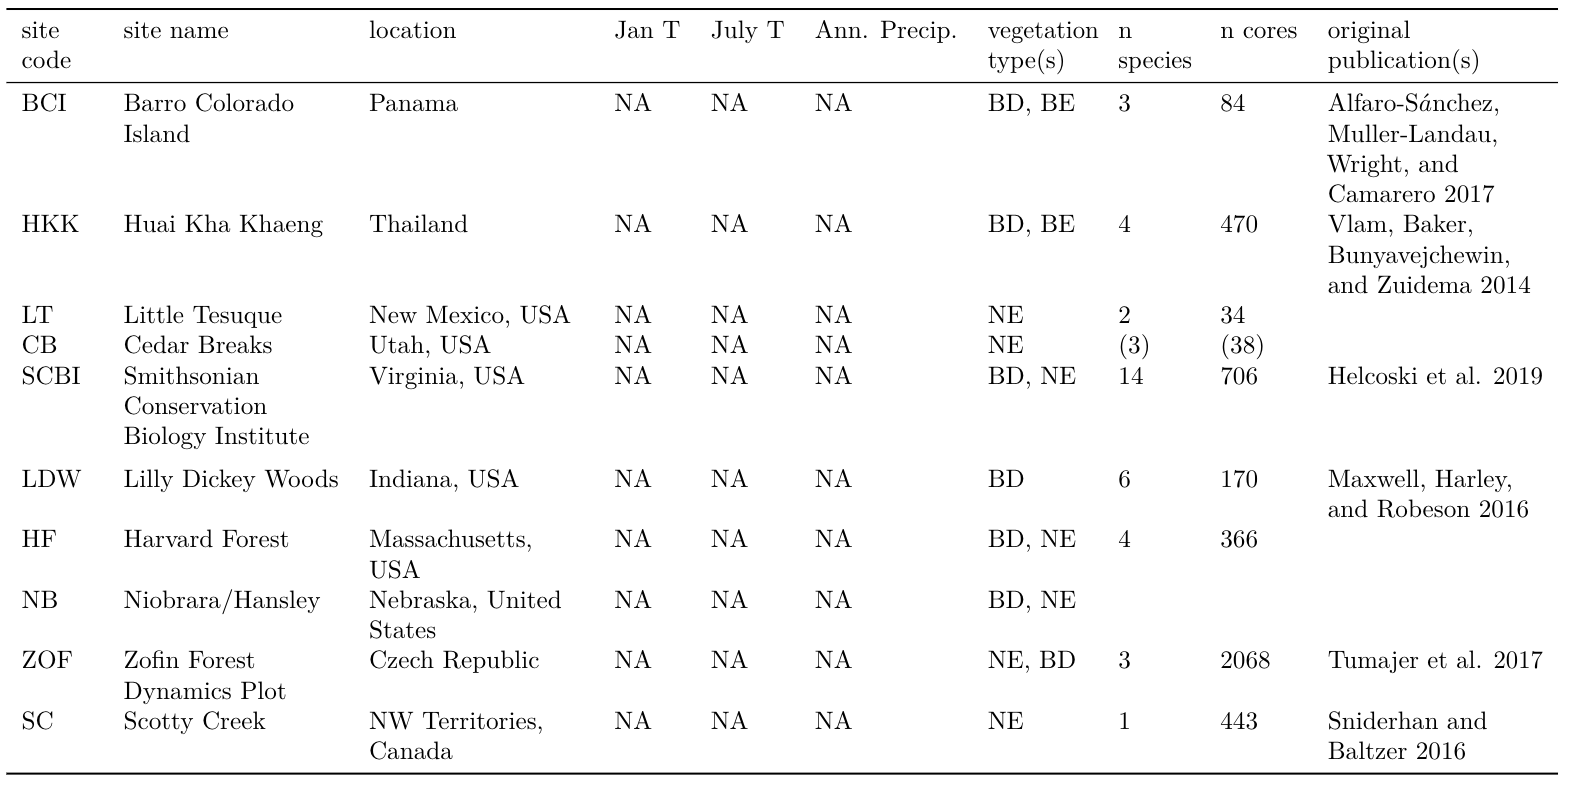
\includegraphics{tables_figures/sites_table.png}

All tree cores were measured and cross-dated by the original researchers
using standard dendrochronological practices. From among the full set of
\emph{\#} original records, we excluded cores for which we detected
errors (e.g., labeling inconsistencies, obvious dating errors) that
could not be resolved before finalizing the analysis (n=\emph{\#}). We
also excluded records that had to be excluded due to insufficient sample
size or anomalous growth patterns, including (1) species with \textless7
cores, (2) cores with \textless30 years of record, (3) contiguous
portions of cores containing large outliers (\(RW\) \textgreater{} mean
plus 5 x SD of \(RW\) for the entire core), and (4) the final 20 years
prior to death of trees cored dead. The final criteria was implemented
to avoid periods of growth decline and potentially altered climate
sensitivity prior to death (Cailleret et al., 2017; DeSoto et al.,
2020). From analyses including \(DBH\) (see below), we further excluded
(1) trees for which we lacked data required to reconstruct \(DBH\), (2)
trees for which there was a significant inconsistency between measured
\(DBH\) and the sum of \(RW\)'s across the core (Appendix S1), and (3)
parts of records where reconstructed \(DBH\) (see below) was represented
by \textless3 conspecific trees. In total, this resulted in inclusion of
\emph{\#} cores, 2234 of which could be included in analyses with
\(DBH\) (Table c(``BCI'', ``BCI'', ``BCI'', ``CB'', ``CB'', ``CB'',
``CB'', ``CB'', ``CB'', ``CB'', ``HF'', ``HF'', ``HF'', ``HF'', ``HKK'',
``HKK'', ``HKK'', ``HKK'', ``LDW'', ``LDW'', ``LDW'', ``LDW'', ``LDW'',
``LDW'', ``NE'', ``NE'', ``NE'', ``LT'', ``LT'', ``SCBI'', ``SCBI'',
``SCBI'', ``SCBI'', ``SCBI'', ``SCBI'', ``SCBI'', ``SCBI'', ``SCBI'',
``SCBI'', ``SCBI'', ``SCBI'', ``SCBI'', ``SCBI'', ``SC''), c(``JACO'',
``TEPA'', ``TRTU'', ``ABBI'', ``PIEN'', ``PIFL'', ``PILO'', ``PIPU'',
``POTR'', ``PSME'', ``ACRU'', ``BEAL'', ``QURU'', ``TSCA'', ``AFXY'',
``CHTA'', ``MEAZ'', ``TOCI'', ``ACSA'', ``CAOV'', ``LITU'', ``QUAL'',
``QUMO'', ``QUVE'', ``BEPA'', ``JUVI'', ``PIPO'', ``PIPO'', ``PIST2'',
``CACO'', ``CAGL'', ``CAOVL'', ``CATO'', ``FAGR'', ``FRAM'', ``FRNI'',
``JUNI'', ``LITU'', ``PIST'', ``QUAL'', ``QUMO'', ``QURU'', ``QUVE'',
``PIMA''), c(12, 18, 23, 22, 12, 13, 17, 15, 17, 11, 18, 13, 74, 32, 39,
28, 46, 45, 35, 9, 15, 10, 10, 9, 28, 29, 59, 10, 7, 15, 39, 25, 15, 76,
66, 12, 30, 106, 36, 66, 67, 70, 81, 442), c(18, 29, 37, 41, 21, 21, 24,
28, 27, 20, 59, 44, 180, 83, 127, 70, 130, 143, 66, 18, 28, 20, 20, 18,
84, 60, 114, 20, 14, 15, 39, 25, 15, 76, 66, 12, 30, 106, 36, 66, 67,
70, 81, 442), c(11, 17, 20, 20, 10, 12, NA, 15, 17, 10, 18, 13, 73, 32,
39, 28, 46, 45, 34, 8, 14, NA, 8, NA, 28, 29, 57, 10, 7, 14, 36, 24, 14,
74, 61, 12, 28, 104, 36, 66, 67, 70, 81, 101), c(17, 26, 31, 37, 15, 20,
NA, 28, 26, 18, 59, 44, 177, 71, 127, 70, 130, 143, 64, 15, 25, NA, 16,
NA, 84, 60, 110, 20, 13, 14, 36, 24, 14, 74, 61, 12, 28, 104, 36, 66,
67, 70, 81, 101), c(``30.2-63.5'', ``22.1-59.5'', ``20.7-43.6'',
``13.9-54.2'', ``14-54.9'', ``17.6-64.1'', NA, ``22.4-50.8'',
``23.6-47.6'', ``20.7-64.2'', ``10.1-22.1'', ``10.2-37.9'', ``19.5-53'',
``10.6-37'', ``20.1-98.7'', ``16-64.6'', ``25.6-98.1'', ``16.6-116.4'',
``9-64.6'', ``NA-NA'', ``NA-NA'', NA, ``NA-NA'', NA, ``NA-NA'',
``16.6-21.5'', ``19.3-63'', ``23.2-52.8'', ``25.7-39.8'',
``10.62-38.52'', ``10.28-52.31'', ``15.11-60.32'', ``12.86-35.95'',
``10.05-41.02'', ``8.11-94.73'', ``11.04-39.2'', ``20.4-76.19'',
``10-91.42'', ``13.92-50.96'', ``11.4-76.73'', ``10.22-84.59'',
``11.07-87.65'', ``16.02-82.33'', ``7-14.9''), c(``2.6-56.4'',
``2.7-49.4'', ``4.8-41.5'', ``0.9-46.4'', ``0.9-33.1'', ``1.5-47.5'',
NA, ``9.5-48.4'', ``4.3-35.4'', ``0.5-41.5'', ``0.9-20.4'', ``0-17.2'',
``1.1-48.3'', ``0-28.4'', ``0.1-81.4'', ``0.2-59.5'', ``3.8-80.3'',
``1.7-80.5'', ``0-52.4'', ``1.4-37.4'', ``1.2-69.4'', NA, ``1.1-52.4'',
NA, ``0-25.5'', ``1.6-18.4'', ``0-39.5'', ``14.6-48.4'', ``4.2-34.4'',
``1.7-32.2'', ``1.6-49.3'', ``2.6-47.2'', ``3.7-28.4'', ``0.1-41.2'',
``0.1-84.4'', ``0.5-27.3'', ``5.6-59.5'', ``0.1-81.1'', ``1.6-45.2'',
``0.3-70.4'', ``0.3-69.5'', ``2.5-79.2'', ``0.5-78.4'', ``0.5-12.5''),
c(``1931-2014'', ``1931-2014'', ``1931-2014'', ``1903-2000'',
``1903-2000'', ``1903-1998'', ``1903-1999'', ``1903-2000'',
``1903-2000'', ``1903-1999'', ``1903-2013'', ``1904-2013'',
``1903-2014'', ``1923-2014'', ``1903-2011'', ``1904-2010'',
``1914-2011'', ``1903-2011'', ``1903-2019'', ``1903-2013'',
``1903-2019'', ``1903-2013'', ``1903-2013'', ``1903-2013'',
``1903-1995'', ``1941-1994'', ``1934-1994'', ``1903-2018'',
``1903-2018'', ``1903-2015'', ``1903-2015'', ``1903-2015'',
``1903-2015'', ``1920-2009'', ``1903-2016'', ``1903-1996'',
``1903-2010'', ``1903-2010'', ``1931-2010'', ``1903-2009'',
``1903-2017'', ``1903-2016'', ``1903-2009'', ``1903-2013'')).

For each year in the tree-ring records, we reconstructed \(DBH\), as
detailed in Appendix S1. In most cases, when a recent \(DBH\)
measurement was available, \(DBH\) was reconstructed from the outside
in. In cases where \(DBH\) was not available, but when we knew that the
core hit pith or could reasonably estimate how far off it was based on
the curvature of the rings (Applequist, 1958; Duncan, 1989), \(DBH\) was
reconstructed from the inside out. In either case, we used allometric
equations between \(DBH\) and bark thickness to account for changes in
bark thickness as the tree grew (Appendix S1; Tables c(``ABBI'',
``ACRU'', ``ACSA'', ``AFXY'', ``BEAL'', ``BEPA'', ``CACO'', ``CAGL'',
``CAOV'', ``CAOVL'', ``CATO'', ``CHTA'', ``FAGR'', ``FRAM'', ``FRNI'',
``JACO'', ``JUNI'', ``JUVI'', ``LITU'', ``MEAZ'', ``PIAB'', ``PIEN'',
``PIFL'', ``PILO'', ``PIMA'', ``PIPO'', ``PIPU'', ``PIST'', ``PIST2'',
``POTR'', ``PSME'', ``QUAL'', ``QUMO'', ``QURU'', ``QUVE'', ``TEPA'',
``TOCI'', ``TRTU'', ``TSCA''), c(``Pinaceae'', ``Sapindaceae'',
``Sapindaceae'', ``Fabaceae'', ``Betulaceae'', ``Betulaceae'',
``Juglandaceae'', ``Juglandaceae'', ``Juglandaceae'', ``Juglandaceae'',
``Juglandaceae'', ``Meliaceae'', ``Fagaceae'', ``Oleaceae'',
``Oleaceae'', ``Bignoniaceae'', ``Juglandaceae'', ``Cupressaceae'',
``Magnoliaceae'', ``Meliaceae'', ``Pinaceae'', ``Pinaceae'',
``Pinaceae'', ``Pinaceae'', ``Pinaceae'', ``Pinaceae'', ``Pinaceae'',
``Pinaceae'', ``Pinaceae'', ``Salicaceae'', ``Pinaceae'', ``Fagaceae'',
``Fagaceae'', ``Fagaceae'', ``Fagaceae'', ``Burseraceae'',
``Meliaceae'', ``Meliaceae'', ``Pinaceae''), c(``Abies bifolia'', ``Acer
rubrum'', ``Acer saccharum'', ``Afzelia xylocarpa'', ``Betula
alleghaniensis'', ``Betula papyrifera'', ``Carya cordiformis'', ``Carya
glabra'', ``Carya ovata'', ``Carya ovalis'', ``Carya tomentosa'',
``Chukrasia tabularis'', ``Fagus grandifolia'', ``Fraxinus americana'',
``Fraxinus nigra'', ``Jacaranada copaia'', ``Juglans nigra'',
``Juniperus virginiana'', ``Liriodendron tulipifera'', ``Melia
azedarach'', ``Picea abies'', ``Picea engelmannii'', ``Pinus flexilis'',
``Pinus longaeva'', ``Picea mariana'', ``Pinus ponderosa'', ``Picea
pungens'', ``Pinus strobus'', ``Pinus strobiformis'', ``Populus
tremuloides'', ``Pseudotsuga menziesii'', ``Quercus alba'', ``Quercus
montana'', ``Quercus rubra'', ``Quercus velutina'', ``Tetragastris
panamensis'', ``Toona ciliata'', ``Trichilia tuberculata'', ``Tsuga
canadensis''), c(``CB'', ``HF'', ``LDW'', ``HKK'', ``HF'', ``NE'',
``SCBI'', ``SCBI'', ``LDW'', ``SCBI'', ``SCBI'', ``HKK'', ``HF, SCBI'',
``LDW, SCBI'', ``SCBI'', ``BCI'', ``SCBI'', ``NE'', ``LDW, SCBI'',
``HKK'', ``HF'', ``CB'', ``CB'', ``CB'', ``SC'', ``NE, LT'', ``CB'',
``HF, SCBI'', ``LT'', ``CB'', ``CB'', ``LDW, SCBI'', ``LDW, SCBI'',
``HF, LDW, SCBI'', ``LDW, SCBI'', ``BCI'', ``HKK'', ``BCI'', ``HF''),
c(``needleleaf'', ``broadleaf'', ``broadleaf'', ``broadleaf'',
``broadleaf'', ``broadleaf'', ``broadleaf'', ``broadleaf'',
``broadleaf'', ``broadleaf'', ``broadleaf'', ``broadleaf'',
``broadleaf'', ``broadleaf'', ``broadleaf'', ``broadleaf'',
``broadleaf'',
"``,''broadleaf``,''broadleaf``,''needleleaf``,''needleleaf``,''needleleaf``,''needleleaf``,''needleleaf``,''needleleaf``,''needleleaf``,''needleleaf``,''needleleaf``,''broadleaf``,''needleleaf``,''broadleaf``,''broadleaf``,''broadleaf``,''broadleaf``,''broadleaf``,''broadleaf``,''broadleaf``,''needleleaf"
), c(``evergreen'', ``deciduous (cold)'', ``deciduous (cold)'',
``deciduous (drought)'', ``deciduous (cold)'', ``deciduous (cold)'',
``deciduous (cold)'', ``deciduous (cold)'', ``deciduous (cold)'',
``deciduous (cold)'', ``deciduous (cold)'', ``brevi-deciduous
(drought)'', ``deciduous (cold)'', ``deciduous (cold)'', ``deciduous
(cold)'', ``deciduous (drought)'', ``deciduous (cold)'', "``,''deciduous
(cold)``,''deciduous
(drought)``,''evergreen``,''evergreen``,''evergreen``,''evergreen``,''evergreen``,''evergreen``,''evergreen``,''evergreen``,''evergreen``,''deciduous
(cold)``,''evergreen``,''deciduous (cold)``,''deciduous
(cold)``,''deciduous (cold)``,''deciduous
(cold)``,''evergreen``,''deciduous
(drought)``,''evergreen``,''evergreen``),
c(''``,''``,''``,''``,''``,''``,''``,''``,''``,''``,''``,''``,''``,''``,''``,''light-demanding``,''``,''``,''``,''light-demanding``,''intermediate``,''``,''``,''``,''``,''``,''``,''``,''``,''``,''``,''``,''``,''``,''``,''shade-tolerant``,''``,''shade-tolerant``,''``),
c(''neglected in CedarBreaks``,''acru in HarvardForest``,''acru in
LillyDickey, acru in LillyDickey``,''neglected in HKK``,''Betula
alleghaniensis in HarvardForest``,''Betula papyrifera in
Nebraska``,''caco in SCBI``,''cagl in SCBI``,''cagl in
LillyDickey``,''caovl in SCBI``,''cato in SCBI``,''neglected in
HKK``,''neglected in HarvardForest, neglected in LillyDickey, neglected
in SCBI``,''Fraxinus ssp. in LillyDickey, fram in SCBI``,''fram in
SCBI``,''JCO in BCI``,''juni in SCBI``,''neglected in Nebraska``,''litu
in LillyDickey, litu in LillyDickey, litu in SCBI``,''neglected in
HKK``,''neglected in HarvardForest, neglected in Zofin``,''Picea
engelmannii in CedarBreaks``,''Pinus monticola in
CedarBreaks``,''neglected in CedarBreaks``,''PIMA in
ScottyCreek``,''Pinus jeffreyi in Little Tesuque, Pinus jeffreyi in
Nebraska``,''neglected in CedarBreaks``,''Pinus strobus in
HarvardForest, pist in SCBI``,''Pinus monticola in Little
Tesuque``,''Populus tremuloides in CedarBreaks``,''Pseudotsuga menziesii
in CedarBreaks``,''qual in LillyDickey, qual in SCBI``,''qupr in
LillyDickey, qupr in SCBI``,''quru in HarvardForest, Quercus rubra in
LillyDickey, quru in SCBI``,''quve in LillyDickey, quve in SCBI``,''TPA
in BCI``,''neglected in HKK``,''TTU in BCI``,''Tsuga canadensis in
HarvardForest"), S4).

Once \(DBH\) had been reconstructed, we used biomass allometries to
estimate the corresponding aboveground biomass and diameter to area
equation to get the corresponding basal area. We then calculated
aboveground biomass growth increments (\(\Delta AGB\)) as
{[}\(AGB_{y+1}-AGB_y\){]} and basal area increment (\(BAI\)) as
{[}\(BAI_{y+1}-BAI_y\){]}. Biomass allometries for temperate and
tropical sites were calculated using the R packages \emph{allo-db}
(Gonzalez-Akre et al.~in prep) and \emph{biomass} (Réjou-Méchain,
Tanguy, Piponiot, Chave, \& Hérault, 2017), respectively.

Monthly climate data for 1901-2019 were obtained from CRU v.4.04
(Harris, Jones, Osborn, \& Lister, 2014; Harris, Osborn, Jones, \&
Lister, 2020), and in some cases corrected based on more local records
(Appendix S2). Variables considered here included average daily minimum,
maximum, and mean temperatures (\(T_{min}\), \(T_{max}\), \(T_{mean}\),
respectively); precipitation (\(PPT\)); and, when deemed reliable
(Appendix S2), potential evapotranspiration (\(PET\)) and precipitation
day frequency (\(PDF\)). \emph{For BCI, we calculated monthly \(PPT\)
and \(PDF\) from daily precipitation readings made on BCI starting in
1929 (Paton, 2019).} All ForestGEO climate records used here are
archived in the ForestGEO Climate Data Portal, \emph{v1.0-alpha}
(Anderson-Teixeira et al., 2020).

\hypertarget{analysis-methods}{%
\subsection{Analysis methods}\label{analysis-methods}}

Our analysis consisted of two main steps: (1) identification of the most
important climate drivers and the time window over which they operate,
and (2) combining \(DBH\) and climate drivers into a multivariate model
(Fig. 1). The analysis was run separately for each site and each
response variable (\(RW\), \(BAI\), or \(\Delta AGB\)).

\begin{figure}
\centering
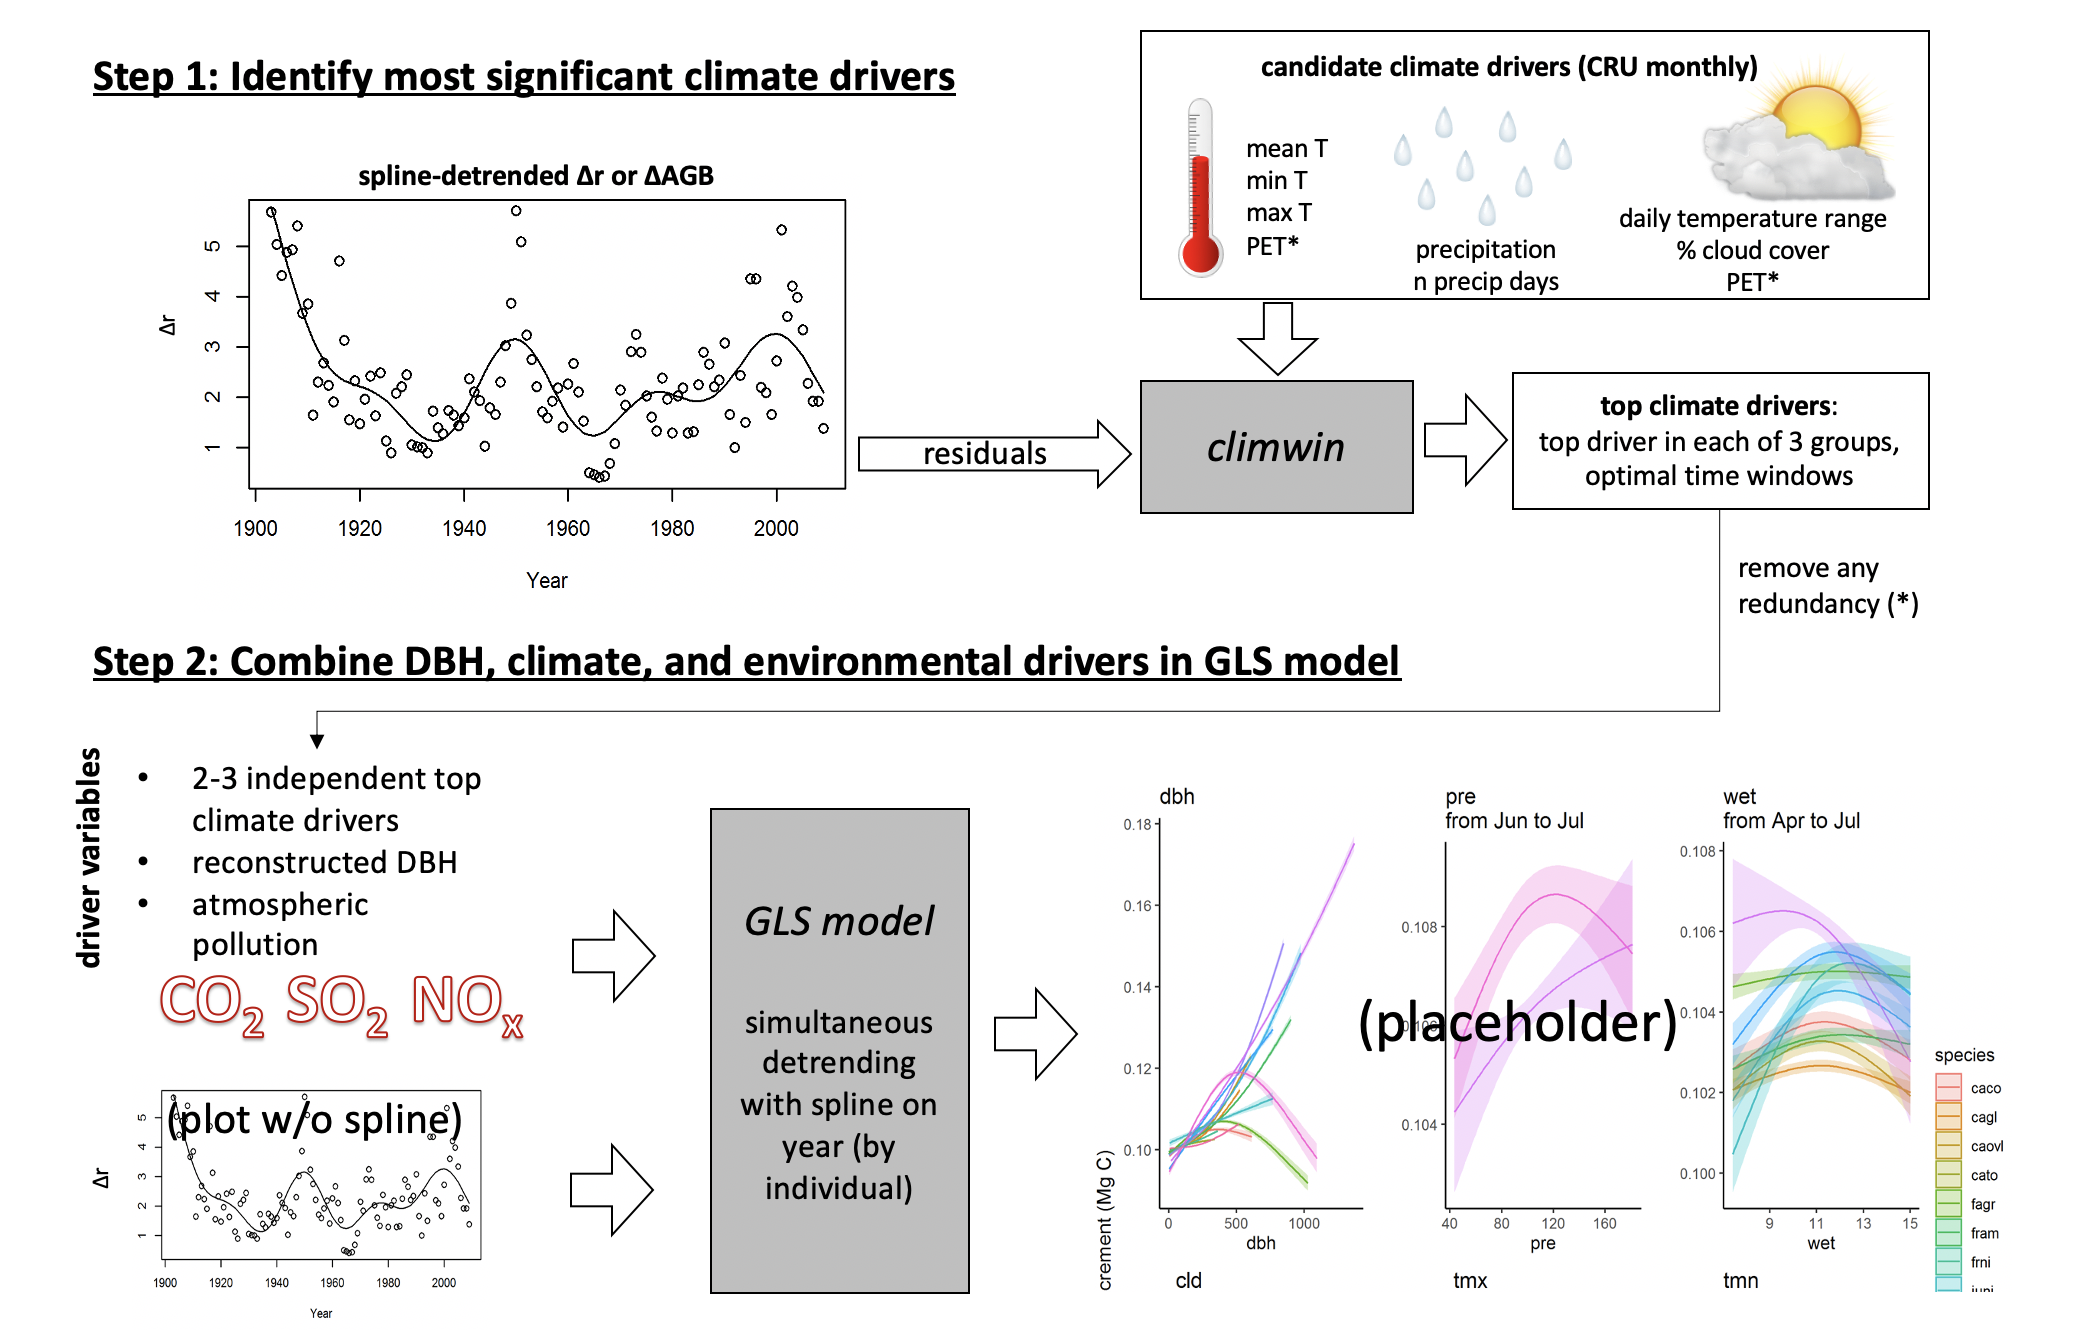
\includegraphics{tables_figures/schematic_figure.png}
\caption{\textbf{Figure 1 \textbar{} DRAFT Schematic illustrating our
analysis process.} This analysis is conducted separately for each site.}
\end{figure}

\hypertarget{identifying-key-climate-drivers}{%
\subsubsection{Identifying key climate
drivers}\label{identifying-key-climate-drivers}}

\textbf{We used the \emph{climwin} package in R (van de Pol et al.,
2016) to identify the most important climate driver and the time window
over which its effect was strongest for each of two categories of
variables: a temperature group (mean, min, and max temperature; PET) and
a precipitation group (precipitation, number of days with
precipitation).} To remove low-frequency variation that most likely
represents responses to non-climatic drivers (\emph{e.g.}, growth and
aging of the tree, change in competitive dynamics, atmospheric
pollution), we detrended the response variables by using a generalized
additive model (GAM) to fit a spline to individual growth records
(\(RW\), \(BAI\), or \(\Delta AGB\)) from each core, thereby producing
residuals. We then used \emph{climwin} to identify the climate variables
most strongly correlated to the residuals of \(RW\), \(BAI\), or
\(\Delta AGB\), specifying quadratic fits to allow for potential
nonlinearities in the climate response. Within \emph{climwin}, we
specified a mixed effects model using species and core identity as
random effects:
\texttt{residual\ growth\ index\ \textasciitilde{}\ {[}climate{]}\ +\ (1\ \textbar{}\ sp)\ +\ (1\ \textbar{}\ treeID)}.
We allowed first-order linear or concave-down second-order polynomial
fits, but ignored any concave-up fits on the basis that these are not
expected biologically and, when identified in initial analyses, often
appeared to be cases of over-fitting
(\textbf{\href{https://github.com/EcoClimLab/ForestGEO-climate-sensitivity/issues/84}{ISSUE
\#84 in ForestGEO-climate-sensitivity}}).

Here, for each permutation, \texttt{climate} specifies one of the
climate drivers in the climate variable group, analyzed over one of all
possible combinations of consecutive months over a 15 month period
ending near the time of cessation of formation of each annual ring
(Table S1).
(\textbf{\href{https://github.com/EcoClimLab/ForestGEO-climate-sensitivity/issues/51}{ISSUE
\#51 in ForestGEO-climate-sensitivity}}) \emph{Climwin} runs all
potential models to select the best fit (lowest AIC), and does k-fold
cross-validation in its computation of AIC to guard against over-fitting
(van de Pol et al., 2016). For each group of candidate climate
variables, we move forward with the best variable over the time window
identified by \emph{climwin} as a candidate climate variable for the
multivariate models.

A challenge to this system arose for the sites that have undergone the
most rapid changes in climate and tree growth: SC and LT, where trees
exhibit significant growth declines attributed to rising temperatures
(Sniderhan \& Baltzer, 2016) and increasing drought (REF), respectively.
\emph{(\href{https://github.com/EcoClimLab/ForestGEO-climate-sensitivity/issues/25}{ISSUE
\#25 in ForestGEO-climate-sensitivity})} Problematically, correlating
tree growth residuals from which climate-driven trends had been removed
against the climate signal with a strong directional trend would not
necessarily identify the most relevant climate drivers. For these sites,
we experimented with three approaches to identifying the most important
climate drivers (1) the method described above, (2) detrending the
climate variables \textbf{(AT:prewhitening?)} prior to the climwin step,
and (3) excluding \emph{decades with the most pronounced climate change}
from the climwin step of the analysis (\emph{sensu} Sniderhan \&
Baltzer, 2016) (Appendix S4). After determining that\ldots{} , here we
present results \emph{(method)}.

We verified that this process identified similar climate variable-month
combinations as what would be identified using traditional methods for
individual species, as detailed in Appendix S1.
(\textbf{\href{https://github.com/EcoClimLab/ForestGEO-climate-sensitivity/issues/35}{ISSUE
\#35 in ForestGEO-climate-sensitivity}})

\hypertarget{combining-drivers-in-gls-model}{%
\subsubsection{Combining drivers in GLS
model}\label{combining-drivers-in-gls-model}}

Having identified candidate climate drivers in temperature and
precipitation variable groups, we next combined climate variables (all
models) and \(DBH\) (models with \(DBH\) and its climate interactions)
in a generalized least squares (GLS) model (Fig. 1). Before running the
models, we checked for collinearity among the candidate variables using
the \emph{vifstep} function (\textbf{REF}) and removed any variable with
a variance inflation factor \textgreater{} 3 (none required removal).
Within the GLS models, our response variables were \(log[\Delta r]\),
\(log[BAI]\), or \(log[\Delta AGB]\). Rather than detrending these
variables to produce residuals, the temporal autocorrelation of
individual tree's growth was accounted for by the specifying an
autocorrelation structure of order 1, with \(Year\) as a continuous time
covariate and \(coreID\) as a grouping factor, in the GLS's model
specification. For each species independently, we ran every combination
of the candidate climate variables and \(DBH\), including both first-
and second-order terms of polynomial for each. For models including
interactive effects of climate and \(DBH\), we included only first-order
linear terms for both \(DBH\) and climate variables.
(\emph{\href{https://github.com/EcoClimLab/ForestGEO-climate-sensitivity/issues/42}{ISSUE
\#42 in ForestGEO-climate-sensitivity}}) Within each of three categories
of models run (climate only, \(DBH\)+climate, \(DBH\) x climate), we
selected as the top model that with the lowest AIC.

\hypertarget{results}{%
\section{Results}\label{results}}

\hypertarget{identifying-climate-drivers}{%
\subsubsection{Identifying climate
drivers}\label{identifying-climate-drivers}}

\textbf{Our process picked out similar climate drivers to what would be
obtained via traditional methods (Figs. 2, }S2\textbf{; Table S5;
Appendix S1), but with the advantage that \emph{climwin} allowed
objective selection of the strongest climate drivers and the time
windows over which they were most influential.} The most commonly
selected variables within the temperature group were \(T_{max}\) and
\(PET\), each of which was identified by climwin as the top
temperature-related driver \emph{at four of the eight sites}.
\(T_{min}\) was the top driver at only \emph{one site (BCI)}, and
\(T_{mean}\) was never identified as the top variable within the
temperature group (Fig. 3). Within the precipitation group,
precipitation amount (\(PPT\)) was identified as the top variable most
frequently (n=\emph{6 of 9} sites), but it was not uncommon that it was
surpassed by precipitation frequency (\(PDF\); n=\emph{3 of 8} sites).
Optimal time windows often coincided with a site's peak growing season
(n= \emph{\# of 10} for temperature variables, \emph{\# of 10} for
precipitation variables), but exceptions were common. At the \emph{5
lowest latitude} sites (BCI, HKK, LT, CB, and SCBI), the optimal window
for precipitation variables spanned \(\ge\) 8 months, ending during the
peak growing months of the year of ring formation. At the \emph{3
highest latitude sites} (HF, ZOF, and SC), the optimal window for
precipitation variables was a short (\(\le\) 3 months) window during the
previous growing season. Optimal windows for temperature variables
tended to be shorter, the longest being a \emph{6}-month period during
the summer (wet season) at HKK. At two of the higher-latitude temperate
sites (HF and Žofín), temperatures were most influential during late
winter/ early spring. There were also a few instances where previous
growing season conditions had the strongest influence.

\begin{figure}
\centering
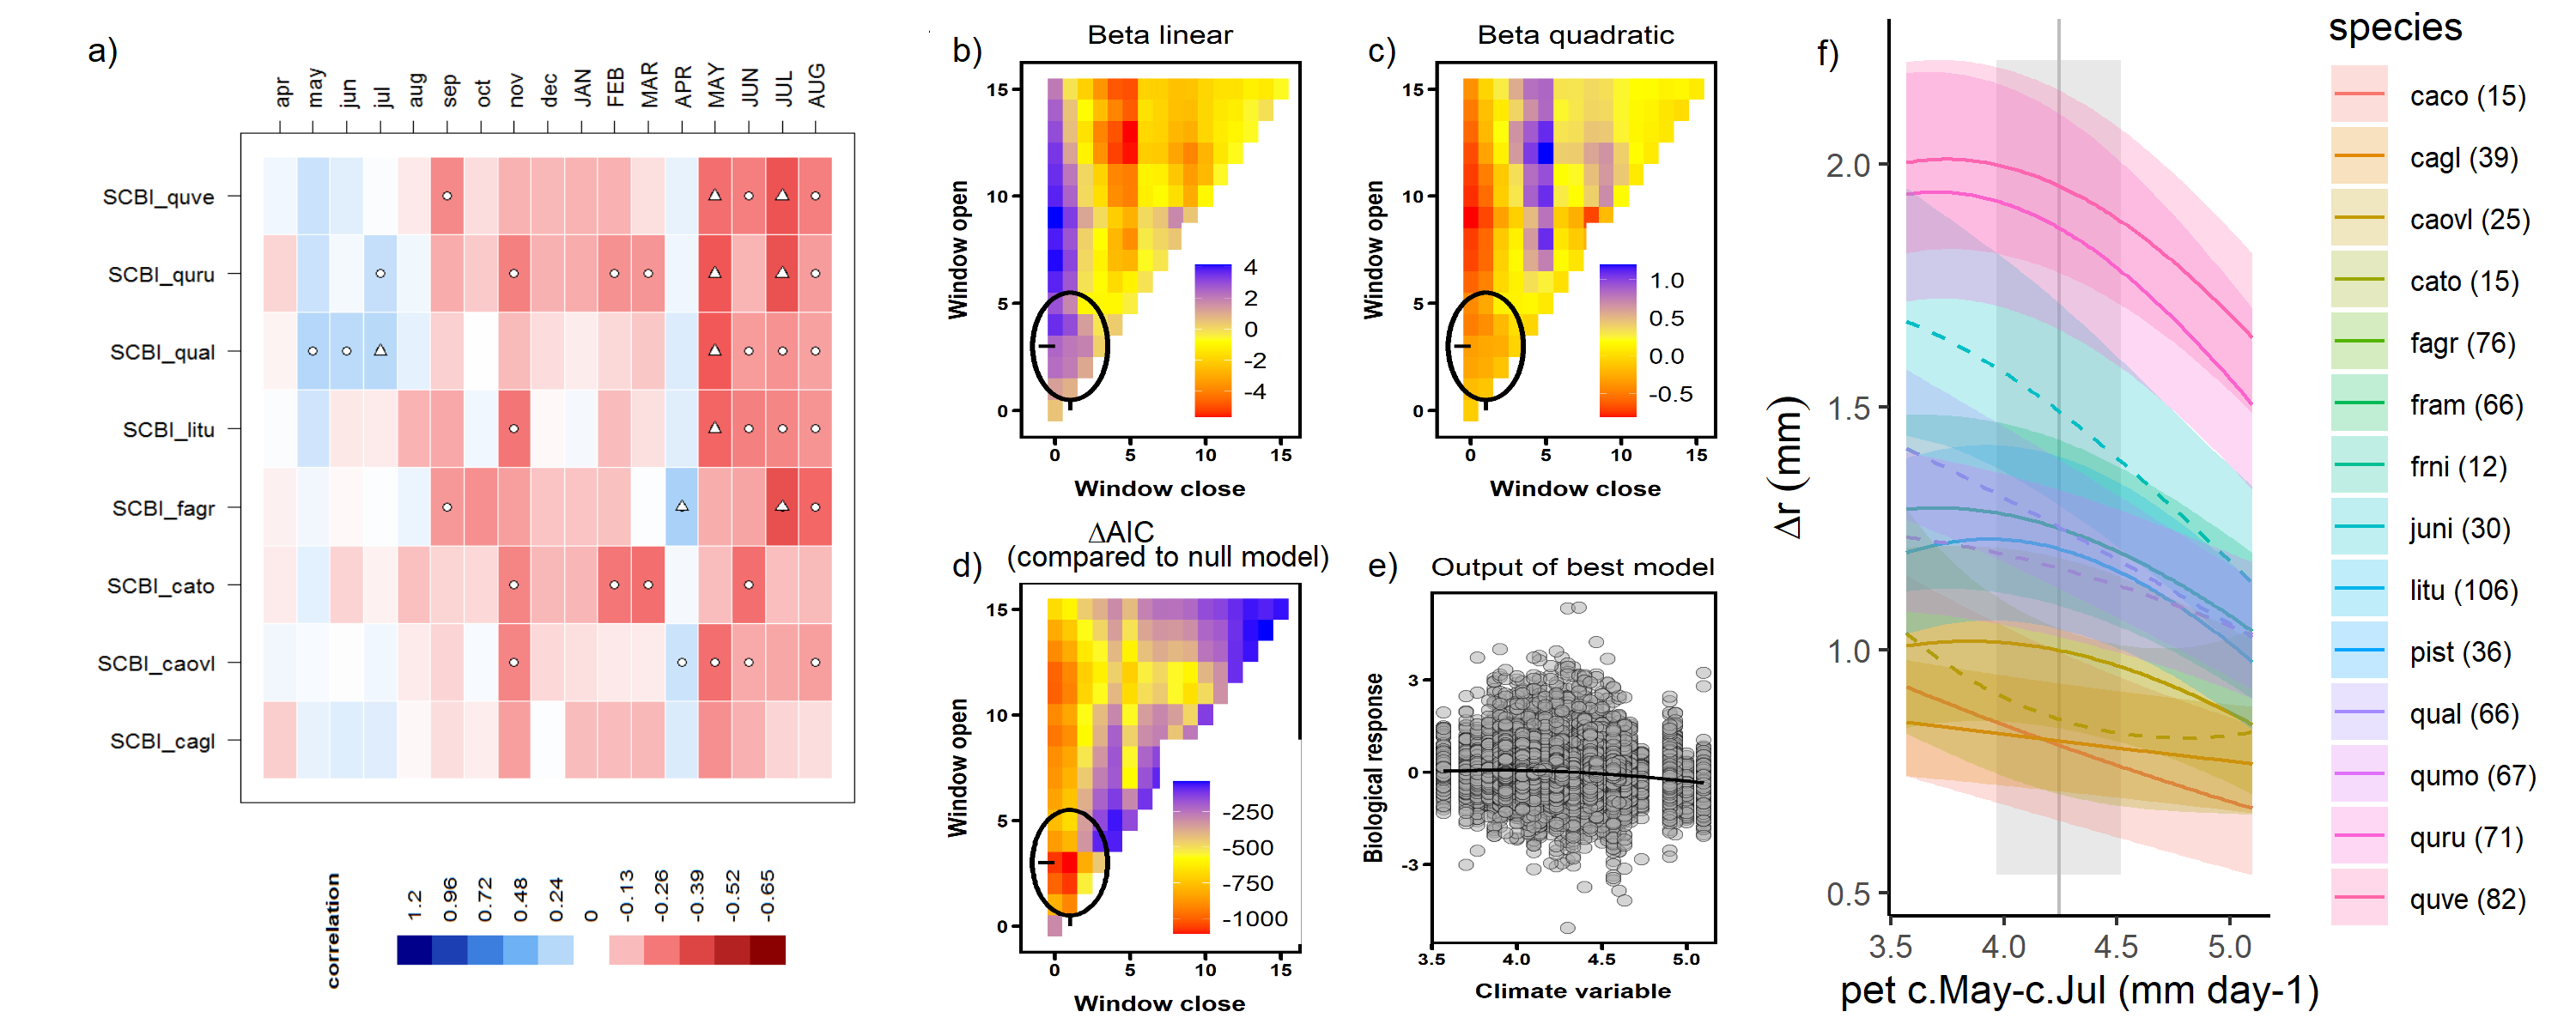
\includegraphics{tables_figures/quilt_comparison.png}
\caption{\textbf{Figure 2 \textbar{} Example comparison of climate
sensitivity derived via traditional methods (}a\textbf{) and our
approach (}b-f\textbf{).} Example is for the sensitivity of 14 species
at SCBI (codes given in Table c(``ABBI'', ``ACRU'', ``ACSA'', ``AFXY'',
``BEAL'', ``BEPA'', ``CACO'', ``CAGL'', ``CAOV'', ``CAOVL'', ``CATO'',
``CHTA'', ``FAGR'', ``FRAM'', ``FRNI'', ``JACO'', ``JUNI'', ``JUVI'',
``LITU'', ``MEAZ'', ``PIAB'', ``PIEN'', ``PIFL'', ``PILO'', ``PIMA'',
``PIPO'', ``PIPU'', ``PIST'', ``PIST2'', ``POTR'', ``PSME'', ``QUAL'',
``QUMO'', ``QURU'', ``QUVE'', ``TEPA'', ``TOCI'', ``TRTU'', ``TSCA''),
c(``Pinaceae'', ``Sapindaceae'', ``Sapindaceae'', ``Fabaceae'',
``Betulaceae'', ``Betulaceae'', ``Juglandaceae'', ``Juglandaceae'',
``Juglandaceae'', ``Juglandaceae'', ``Juglandaceae'', ``Meliaceae'',
``Fagaceae'', ``Oleaceae'', ``Oleaceae'', ``Bignoniaceae'',
``Juglandaceae'', ``Cupressaceae'', ``Magnoliaceae'', ``Meliaceae'',
``Pinaceae'', ``Pinaceae'', ``Pinaceae'', ``Pinaceae'', ``Pinaceae'',
``Pinaceae'', ``Pinaceae'', ``Pinaceae'', ``Pinaceae'', ``Salicaceae'',
``Pinaceae'', ``Fagaceae'', ``Fagaceae'', ``Fagaceae'', ``Fagaceae'',
``Burseraceae'', ``Meliaceae'', ``Meliaceae'', ``Pinaceae''), c(``Abies
bifolia'', ``Acer rubrum'', ``Acer saccharum'', ``Afzelia xylocarpa'',
``Betula alleghaniensis'', ``Betula papyrifera'', ``Carya cordiformis'',
``Carya glabra'', ``Carya ovata'', ``Carya ovalis'', ``Carya
tomentosa'', ``Chukrasia tabularis'', ``Fagus grandifolia'', ``Fraxinus
americana'', ``Fraxinus nigra'', ``Jacaranada copaia'', ``Juglans
nigra'', ``Juniperus virginiana'', ``Liriodendron tulipifera'', ``Melia
azedarach'', ``Picea abies'', ``Picea engelmannii'', ``Pinus flexilis'',
``Pinus longaeva'', ``Picea mariana'', ``Pinus ponderosa'', ``Picea
pungens'', ``Pinus strobus'', ``Pinus strobiformis'', ``Populus
tremuloides'', ``Pseudotsuga menziesii'', ``Quercus alba'', ``Quercus
montana'', ``Quercus rubra'', ``Quercus velutina'', ``Tetragastris
panamensis'', ``Toona ciliata'', ``Trichilia tuberculata'', ``Tsuga
canadensis''), c(``CB'', ``HF'', ``LDW'', ``HKK'', ``HF'', ``NE'',
``SCBI'', ``SCBI'', ``LDW'', ``SCBI'', ``SCBI'', ``HKK'', ``HF, SCBI'',
``LDW, SCBI'', ``SCBI'', ``BCI'', ``SCBI'', ``NE'', ``LDW, SCBI'',
``HKK'', ``HF'', ``CB'', ``CB'', ``CB'', ``SC'', ``NE, LT'', ``CB'',
``HF, SCBI'', ``LT'', ``CB'', ``CB'', ``LDW, SCBI'', ``LDW, SCBI'',
``HF, LDW, SCBI'', ``LDW, SCBI'', ``BCI'', ``HKK'', ``BCI'', ``HF''),
c(``needleleaf'', ``broadleaf'', ``broadleaf'', ``broadleaf'',
``broadleaf'', ``broadleaf'', ``broadleaf'', ``broadleaf'',
``broadleaf'', ``broadleaf'', ``broadleaf'', ``broadleaf'',
``broadleaf'', ``broadleaf'', ``broadleaf'', ``broadleaf'',
``broadleaf'',
"``,''broadleaf``,''broadleaf``,''needleleaf``,''needleleaf``,''needleleaf``,''needleleaf``,''needleleaf``,''needleleaf``,''needleleaf``,''needleleaf``,''needleleaf``,''broadleaf``,''needleleaf``,''broadleaf``,''broadleaf``,''broadleaf``,''broadleaf``,''broadleaf``,''broadleaf``,''broadleaf``,''needleleaf"
), c(``evergreen'', ``deciduous (cold)'', ``deciduous (cold)'',
``deciduous (drought)'', ``deciduous (cold)'', ``deciduous (cold)'',
``deciduous (cold)'', ``deciduous (cold)'', ``deciduous (cold)'',
``deciduous (cold)'', ``deciduous (cold)'', ``brevi-deciduous
(drought)'', ``deciduous (cold)'', ``deciduous (cold)'', ``deciduous
(cold)'', ``deciduous (drought)'', ``deciduous (cold)'', "``,''deciduous
(cold)``,''deciduous
(drought)``,''evergreen``,''evergreen``,''evergreen``,''evergreen``,''evergreen``,''evergreen``,''evergreen``,''evergreen``,''evergreen``,''deciduous
(cold)``,''evergreen``,''deciduous (cold)``,''deciduous
(cold)``,''deciduous (cold)``,''deciduous
(cold)``,''evergreen``,''deciduous
(drought)``,''evergreen``,''evergreen``),
c(''``,''``,''``,''``,''``,''``,''``,''``,''``,''``,''``,''``,''``,''``,''``,''light-demanding``,''``,''``,''``,''light-demanding``,''intermediate``,''``,''``,''``,''``,''``,''``,''``,''``,''``,''``,''``,''``,''``,''``,''shade-tolerant``,''``,''shade-tolerant``,''``),
c(''neglected in CedarBreaks``,''acru in HarvardForest``,''acru in
LillyDickey, acru in LillyDickey``,''neglected in HKK``,''Betula
alleghaniensis in HarvardForest``,''Betula papyrifera in
Nebraska``,''caco in SCBI``,''cagl in SCBI``,''cagl in
LillyDickey``,''caovl in SCBI``,''cato in SCBI``,''neglected in
HKK``,''neglected in HarvardForest, neglected in LillyDickey, neglected
in SCBI``,''Fraxinus ssp. in LillyDickey, fram in SCBI``,''fram in
SCBI``,''JCO in BCI``,''juni in SCBI``,''neglected in Nebraska``,''litu
in LillyDickey, litu in LillyDickey, litu in SCBI``,''neglected in
HKK``,''neglected in HarvardForest, neglected in Zofin``,''Picea
engelmannii in CedarBreaks``,''Pinus monticola in
CedarBreaks``,''neglected in CedarBreaks``,''PIMA in
ScottyCreek``,''Pinus jeffreyi in Little Tesuque, Pinus jeffreyi in
Nebraska``,''neglected in CedarBreaks``,''Pinus strobus in
HarvardForest, pist in SCBI``,''Pinus monticola in Little
Tesuque``,''Populus tremuloides in CedarBreaks``,''Pseudotsuga menziesii
in CedarBreaks``,''qual in LillyDickey, qual in SCBI``,''qupr in
LillyDickey, qupr in SCBI``,''quru in HarvardForest, Quercus rubra in
LillyDickey, quru in SCBI``,''quve in LillyDickey, quve in SCBI``,''TPA
in BCI``,''neglected in HKK``,''TTU in BCI``,''Tsuga canadensis in
HarvardForest")) to potential evapotranspiration (\(PET\)). Panel
(\textbf{a}) shows a matrix of Pearson correlations between ring-width
index and monthly climate variables (using the chronologies of Helcoski
et al.~2019). Black rectangle represents the period selected by
\emph{climwin} as the most influential window. Panels (\textbf{b-d})
give statistics for time windows tested in \emph{climwin}, where window
open and close indicate months prior to current August, and cells across
the lower diaganol indicate single-month tests (akin to panel
\textbf{a}). Panels (\textbf{b}) and (\textbf{c}) give values of linear
and quadratic terms for each time window, and (\textbf{d}) gives the
\(\Delta AIC\) for each. The time window with the minimum \(\Delta AIC\)
(0-3 months prior to August, or May-July; black circles), was identified
as the optimal window. Panel (\textbf{e}) shows the correlation of
individual-level residuals to PET, with the function fit in
\emph{climwin}. Finally, panel (\textbf{f}) shows GLS model output,
where \(PET\) was a candidate driver variable (along with \(PPT\);
\(DBH\) not included in this model). Plotted are responses of species
for which \(PET\) was included in the top model, with best-fit
polynomials plotted with solid lines when both first- and second-order
terms are significant, dashed lines when only one term is significant,
and dotted lines when neither is significant. Transparent ribbons
indicate 95 PERCENTconfidence intervals.}
\end{figure}

\textbf{Across the three metrics of growth, the ``landscape'' of climate
effects over various time windows was generally similar, but the optimal
time window or even the top climate variable sometimes differed (Figs.
}S2\textbf{-}S4\textbf{).} Specifically, \(RW\), \(BAI\), and
\(\Delta AGB\) consistently exhibited similar strength of correlation
and direction of response to climate variables within the temperature
and precipitation variable groups. In some cases (n= \# of \#), both the
optimal climate variable and time window were identical across growth
metrics (e.g., Fig. \textbf{S2}). In \#cases, \emph{climwin} identified
the same climate variable but different (sometimes overlapping) time
windows. In \emph{2} cases (precipitation variable group at LT,
temperature variable group at HKK), \emph{climwin} identified different
climate variables, but identical or overlapping time windows (e.g., Fig.
\textbf{S3}). Finally, in \emph{2} cases of variables that had only weak
effects and mixed responses among species in the final models
(temperature variable group at BCI, precipitation variable group at HF;
Figs. 3, \textbf{S5, S11}), \emph{climwin} identified different climate
variables and different time windows (e.g., Fig. \textbf{S4}).
Henceforth, we focus on the climate drivers identified when \(RW\) was
the growth metric and for the full set of cores (i.e., including those
for which \(DBH\) could not be reconstructed.)

\begin{figure}
\centering
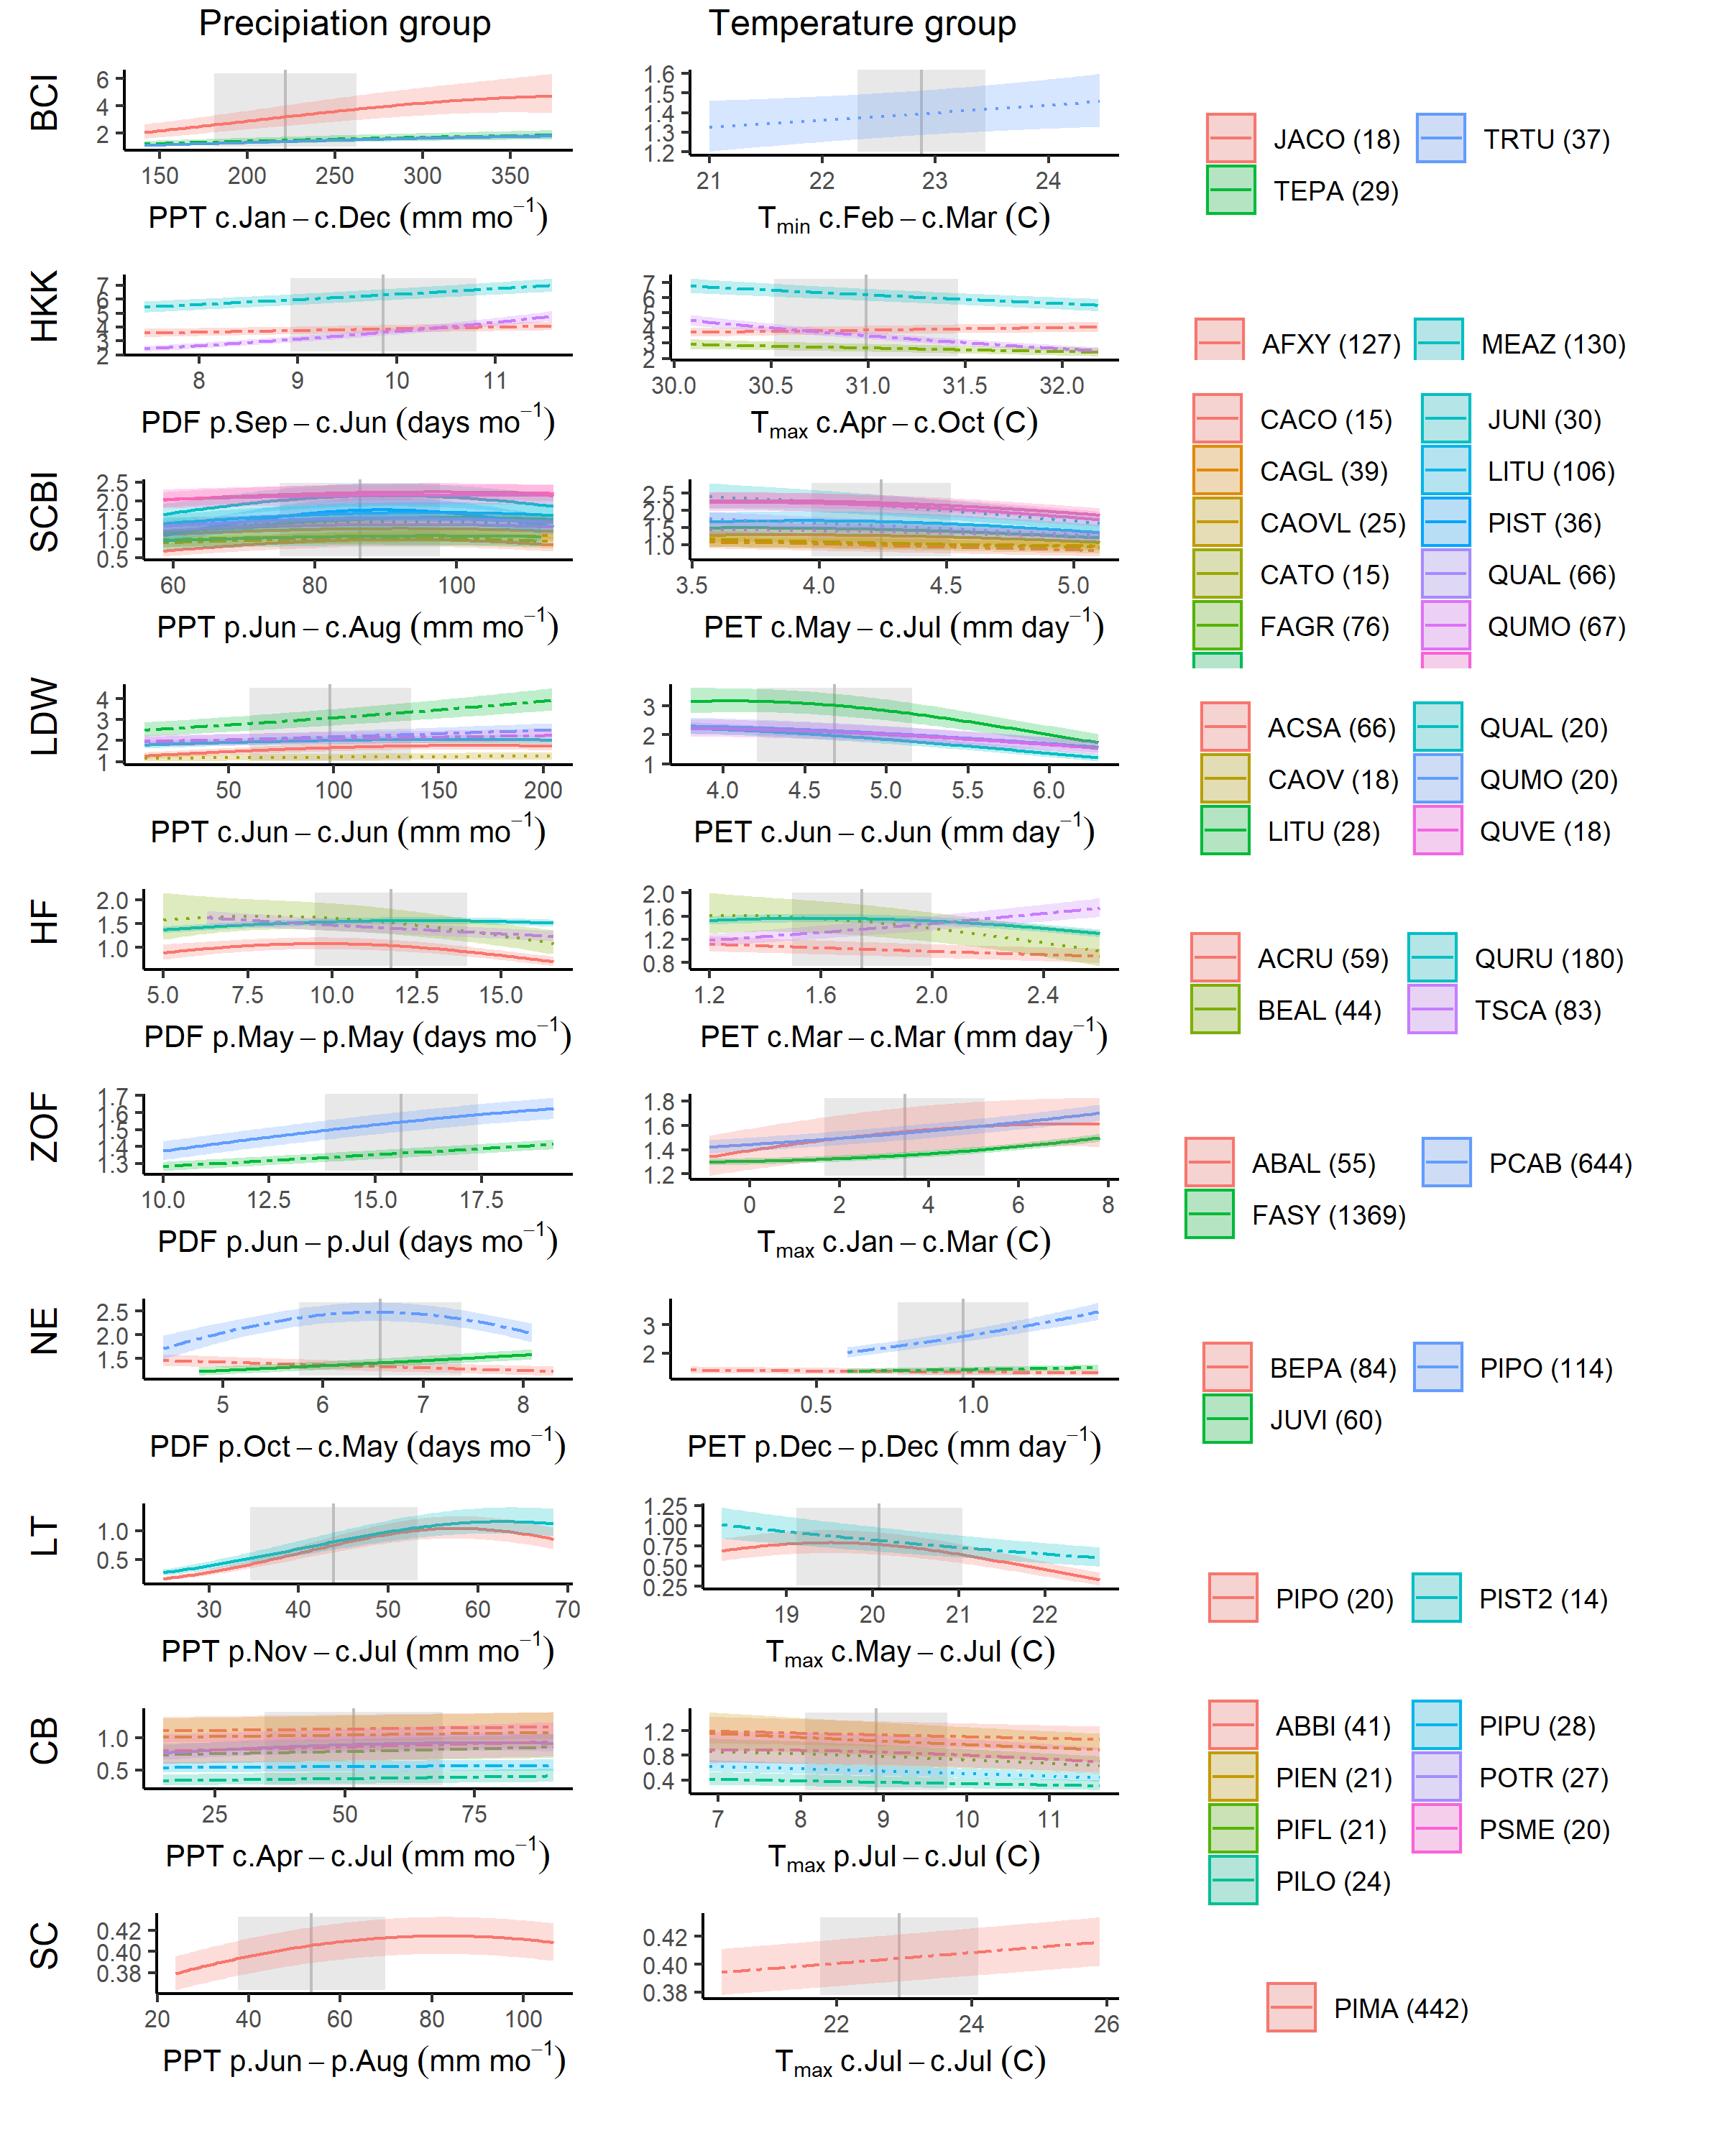
\includegraphics{tables_figures/pre_temp_groups.png}
\caption{\textbf{Figure 3 \textbar{} Species-level responses of \(RW\)
to climwin-selected variables in precipitation and temperature variable
groups.} For each species (color-coded as in Fig. 4), relationships are
plotted if included in top model. For each relationship shown, other
terms in the model are held constant at their median. Best-fit
polynomials are plotted with solid lines when both first- and
second-order terms are significant (t-test's p-value \textless0.05),
dashed lines when only one term is significant, and dotted lines when
neither is significant. Transparent ribbons indicate 95 PERCENT
confidence intervals. Vertical grey lines indicate the long-term mean
for the climate variable, shading indicates 1 SD. (THIS FIGURE WILL
PROBABLY CHANGED INTO A 4COL X 5 ROW MATIX, DROPPING SPECIES KEY, WHICH
CAN BE SEEN IN OTHER FIGURES)}
\end{figure}

\hypertarget{climate-sensitivity}{%
\subsubsection{Climate sensitivity}\label{climate-sensitivity}}

Precipitation responses were included in the best model at all sites and
\emph{for all but \# species} (Fig. 3). Responses were most commonly
positive, and were most pronounced at the driest site (LT).
Precipitation terms included in top models were non-linear \#\% of the
time, and significantly better than first-order linear model \#\% of the
time. In some cases, the non-linearity was quite pronounced (e.g., LT),
with the most common pattern (\#\%) being a decelerating increase.

Temperature responses were included in the best model at all sites and
\emph{for the majority of species} (Fig. 3). Specifically, a temperature
term was included in the best model for \# of \# site-species
combinations, with at least one polynomial term significant for \#, and
both for \#. Among the relationships with at least one significant term,
responses shifted from near-universally negative below 40\(^\circ\)
latitude (exception: AFXY at HKK) to positive above 45\(^\circ\)
latitude. Harvard Forest, at 42.5\(^\circ\) N, exhibited a mix of
responses. \emph{(It will be interesting to see what happens with Indian
Creek, at 42.8 latitude.)} \emph{(Note that Scotty Creek was previously
positive, later shifted negative;
\href{https://github.com/EcoClimLab/ForestGEO-climate-sensitivity/issues/25}{ISSUE
\#25 in ForestGEO-climate-sensitivity})} Temperature terms included in
top models were non-linear \#\% \emph{(most)} of the time, and
significantly better than first-order linear model \#\% of the time.

\hypertarget{influence-of-dbh}{%
\subsubsection{Influence of DBH}\label{influence-of-dbh}}

\textbf{All three growth metrics, \(RW\), \(BAI\), and \(\Delta AGB\),
varied with \(DBH\) for most species at all sites (Fig. 4).} While
\(RW\) varied significantly with \(DBH\) for the majority of
species-site combinations (n= \# of \#; Table \textbf{S\#}), there was
substantial variation in these trends, with patterns mixed across both
forests and species within a single stand (Fig. 4). On one end of the
spectrum, \emph{Melia azedarach} at HKK had extremely rapid growth at
small \(DBH\), with \(RW\) ranging up to \textasciitilde15mm
yr\textsuperscript{-1}, followed by fairly rapid declines with
increasing \(DBH\). Similar patterns of approximately exponential
decline in \(RW\) with \(DBH\) were observed for conifer species at
Little Tesuque and Scotty Creek--both relatively open forests--and a
number of species in mesic temperate forests (Fig. 4). At the other end
of the spectrum, a number of species at sites where they presumably
established under closed-canopy conditions (e.g., \emph{Fagus} at SCBI
and Žofín) had \(RW\) \textless1 mm yr\textsuperscript{-1} at small
\(DBH\), increased to peak \(RW\) between \# and \# cm \(DBH\), and
subsequently declined.

\textbf{The variable patterns in \(RW\) with \(DBH\) translated into
differences in variation in \(BAI\) and \(\Delta AGB\) with \(DBH\),
although trends in both of these were more consistent across sites and
species, typically increasing to a peak at intermediate \(DBH\) and then
declining (Fig. 4).}

\begin{figure}
\centering
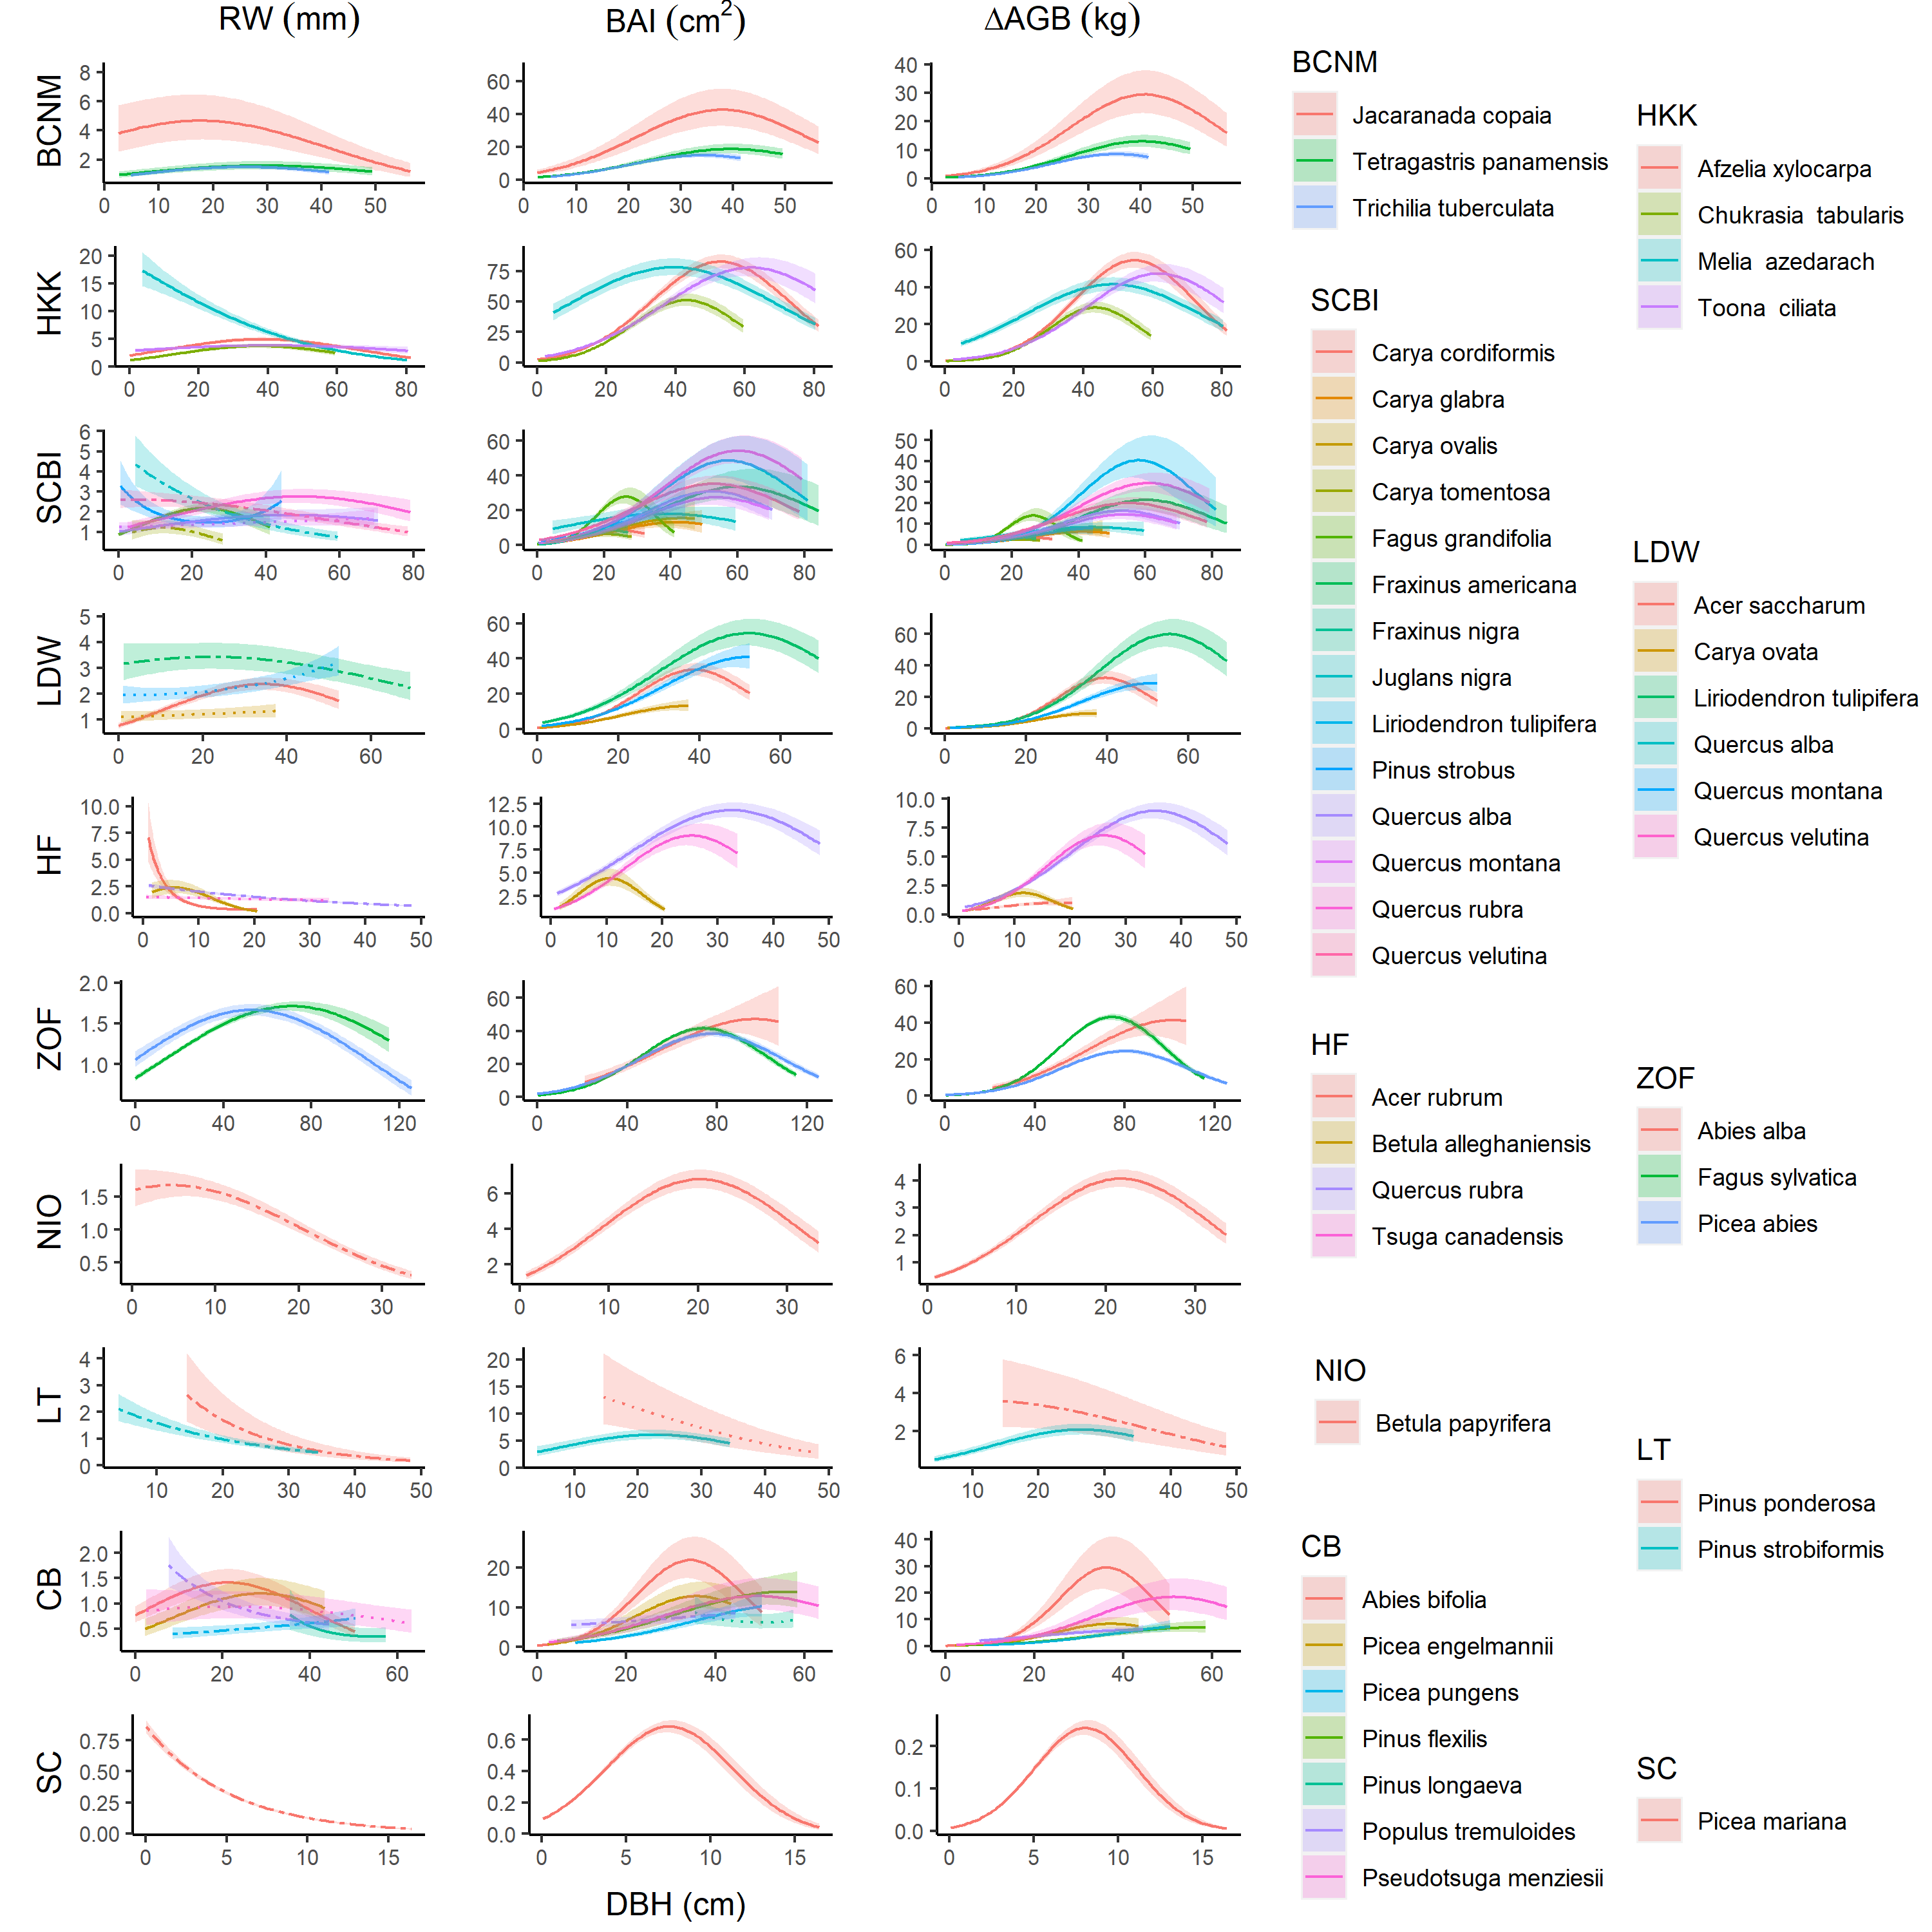
\includegraphics{tables_figures/DBH_responses.png}
\caption{\textbf{Figure 4 \textbar{} Growth sensitivity to DBH: (a)
\(RW\), (b) \(BAI\), (c) \(\Delta AGB\).} Relationships for species are
plotted when included in the top model. Other terms in the model are
held constant at their median. Best-fit polynomials are plotted with
solid lines when both first- and second-order terms are significant
(t-test's p-value \textless0.05), DASHED lines when only one term is
significant, and dotted lines when neither is significant. Transparent
ribbons indicate 95 PERCENTconfidence intervals.}
\end{figure}

\hypertarget{additive-and-interactive-effects-of-climate-and-dbh}{%
\subsubsection{Additive and interactive effects of climate and
DBH}\label{additive-and-interactive-effects-of-climate-and-dbh}}

\textbf{Both DBH and climate were included in the majority of top
models, regardless of the growth metric used.} Specifically, \(DBH\) was
included in \#\% of top models for \(RW\), \#\% of top models for
\(BAI\), and \#\% of top models for \(\Delta AGB\). In general, \(DBH\)
explained more variation in growth rates than did climate (Fig. 5).

\textbf{The relative importance of \(DBH\) and climate shifted across
growth metrics and climates (Figs. 5, }S5\textbf{-}S14\textbf{).} The
relative importance of \(DBH\) tended to be least for \(RW\),
intermediate for \(BAI\), and highest for \(\Delta AGB\) (e.g., at SCBI;
Fig. 5). However, there were exceptions, particularly when \(RW\)
decreased steeply with \(DBH\) (e.g., at Little Tesuque; Fig. 5). The
relative importance of climate was modest at sites including SCBI (Fig.
5), HF (Fig. \textbf{S11}), and SC (Fig. \textbf{S14}), and stronger at
sites including LT (Fig. 5) and BCI (Fig. \textbf{S5}).

\begin{figure}
\centering
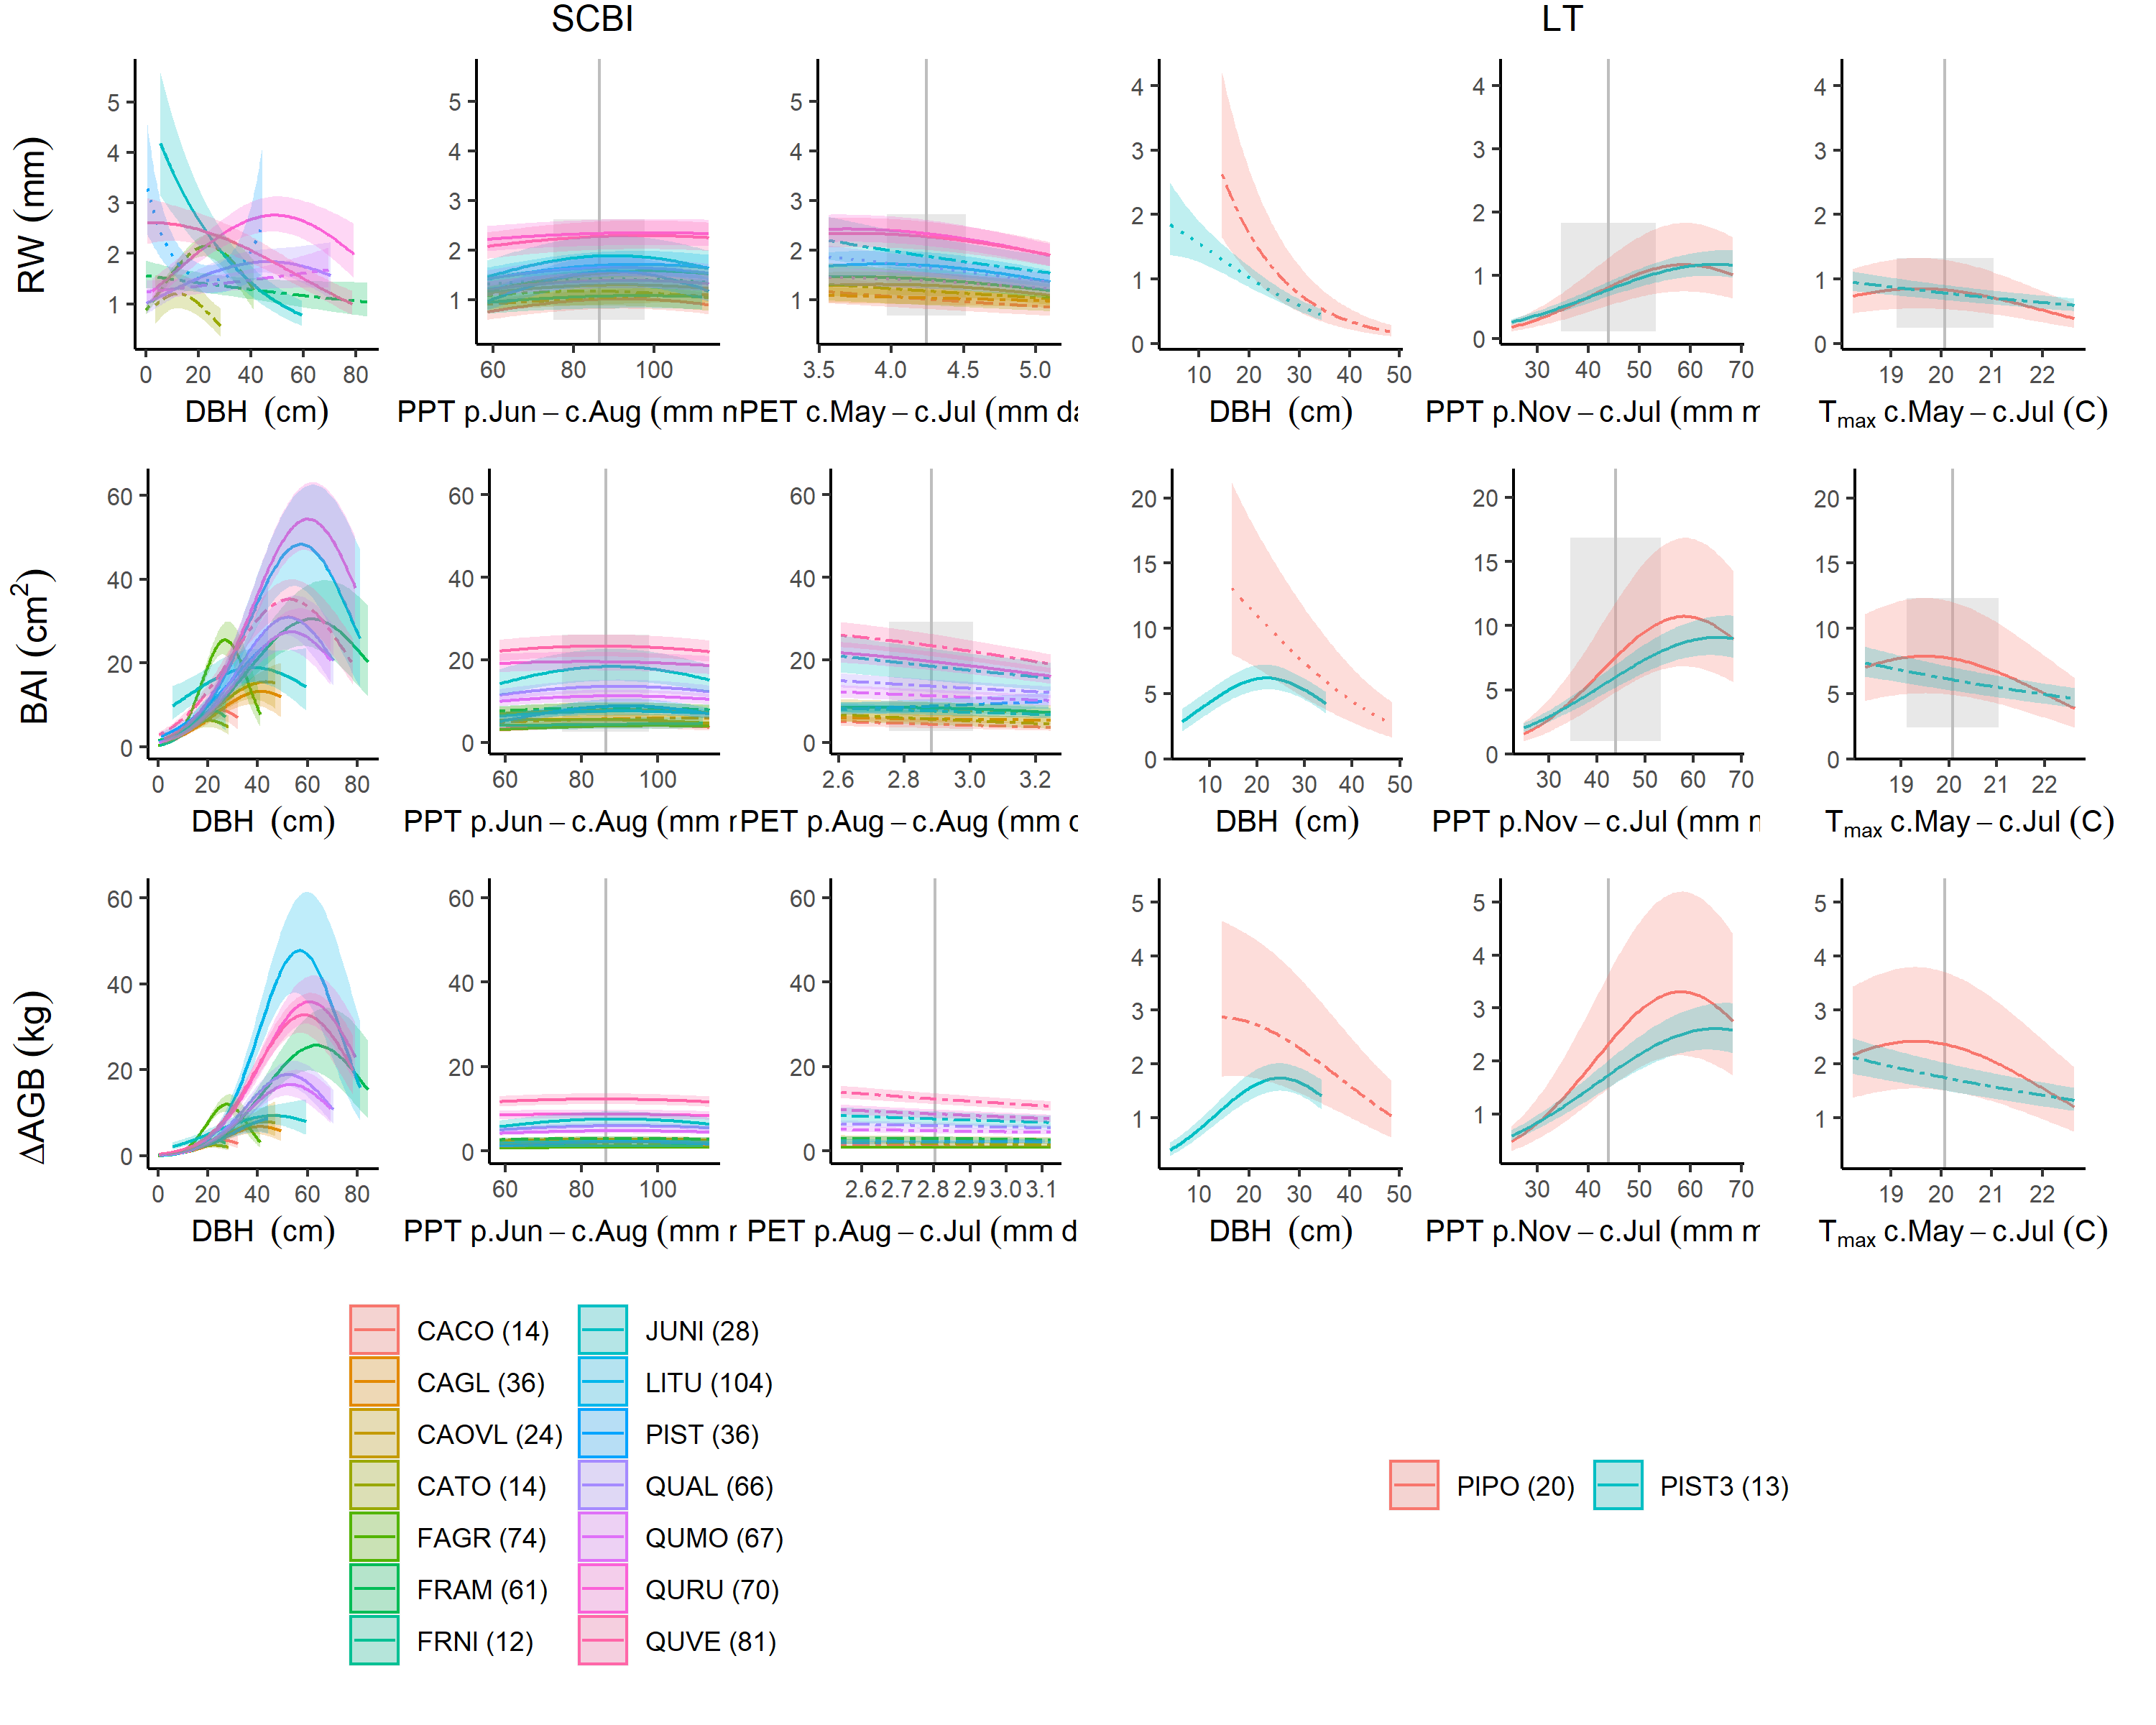
\includegraphics{tables_figures/show_case_response_plots.png}
\caption{\textbf{Figure 5 \textbar{} Comparison of full top models for
each growth metric (\(RW\), \(BAI\), \(\Delta AGB\)) at sites where
climatic controls are strong (Little Tesuque, left panel) and modest
(SCBI, right panel).} Plotted are best fit models for each species, with
transparent ribbons indicating 95 PERCENTconfidence intervals. For
climate variables, best-fit polynomials are plotted with solid lines
when both first- and second-order terms are significant, dashed lines
when only one term is significant, and dotted lines when neither is
significant. Vertical grey lines indicate the long-term mean for the
climate variable, shading indicates 1 SD.}
\end{figure}

\textbf{Interactive effects of \(DBH\) and climate were found for \#\%
of species-variable combinations}. Interactions were significant for
over half of \(DBH\)-precipitation variable interactions for all three
growth metrics (\emph{51\% for all}; Table S6). The majority (\#\%) of
these interactions were positive, indicating that larger trees generally
respond more positively (or less negatively) to precipitation or it's
frequency (Fig. \textbf{6?}). Interactions between temperature variables
and \(DBH\) were significant for \emph{\textasciitilde40\%} of cases
considered (Table S6). The majority (\#\%) of these interactions were
positive, indicating that larger trees generally respond less negatively
(or more positively) to \(T_{max}\) or \(PET\) (Fig. \textbf{6?}).

\textbf{figure on climate - DBH interactions?} (\emph{See
\href{https://github.com/EcoClimLab/ForestGEO-climate-sensitivity/issues/42}{ISSUE
\#42 in ForestGEO-climate-sensitivity}})

\hypertarget{discussion}{%
\section{Discussion}\label{discussion}}

\textbf{We present a new method that allows simultaneous consideration
of the effects of objectively determined principle climate drivers and
tree size on annual growth.} Results are broadly consistent with those
obtained by traditional methods, but offer several new insights.

\hypertarget{corroboration-of-insight-from-conventional-methods}{%
\subsection{corroboration of insight from conventional
methods}\label{corroboration-of-insight-from-conventional-methods}}

\emph{( more objective approach to produce similar results to what has
been shown using more conventional methods)} \emph{(for identigying
climate variables\ldots{} Is the benefit of the new approach that it is
a more objective way to reach the same interpretation, or are there
cases when it would produce a different interpretation?)}

\hypertarget{new-insight}{%
\subsection{new insight}\label{new-insight}}

\emph{(could potentially provide new insight that would not be expected
using more conventional methods. It would be useful if there are
examples from the analysis in this paper that could clearly illustrate
new insight that would not have been found with conventional methods. )}

\hypertarget{future-challenges}{%
\subsection{future challenges (?)}\label{future-challenges}}

\emph{(still face a problem when future climate is outside of the range
of values used to model the climate-growth relationship. )}

\emph{(growth rate should respond strongly to a tree's relative DBH
within a site, which we don't have going back in time)}

\emph{Climate sensitivity}

Ideas to discuss:

\begin{itemize}
\item
  \(T_{max}\) and \(PET\) tend to be better variables than the more
  commonly used \(T_{mean}\)
\item
  trees tend to be sensitive to water over longer time scales (makes
  sense-- lags caused by soil moisture storage)
\item
  temperature sensitivity shifts from neg in warm climates to positive
  in cold climates (although Sniderhan \& Baltzer (2016) shows that the
  effect shifted to negative as warming progressed)
\item
  additive effects are prevalent and should not be overlooked
\item
  nonlinear effects are prevalent
\item
  species climate sensitivity models could be improved by fitting
  climwin individually be species.
\end{itemize}

\emph{Influence of DBH}

\textbf{The diversity of growth trends in relation to \(DBH\) observed
here (Fig. 4) is largely attributable to species ecology and stand
history (Fig. 4).} On one end of the spectrum, species that would have
established in fairly open conditions--\emph{i.e.}, shade-intolerant
species and those at sites with more open canopies (e.g., LT, SC)--
exhibited rapid initial growth followed by a roughly exponential
decline. The most pronounced example of this pattern was \emph{Melia
azedarach} --a highly shade-intolerant species that generally
establishes in the open (Baker \& Bunyavejchewin, 2006) and was sampled
opportunistically outside the ForestGEO plot at HKK (Vlam, Baker,
Bunyavejchewin, \& Zuidema, 2014), where it presumably established under
open conditions. Such patterns are consistent with dendrochronology's
``textbook'' patterns, which have been derived primarily from open-grown
trees (\emph{DENDRO\_REFS: See refs in Biondi and Qeadan 2008. Tree-Ring
Research 64:81-96.}). On the other end of the spectrum, shade-tolerant
species (e.g.~\emph{Fagus} at SCBI and Žofín) exhibited initially low,
but increasing, \(RW\). This pattern is consistent with patterns
observed in stand-level census data from closed-canopy forests,
including several in this analysis, where \(RW\) increases continuously
with \(DBH\) {[}Muller-Landau et al. (2006); Anderson-Teixeira,
McGarvey, et al. (2015); Piponiot et al.~in prep{]}. While the low
community mean \(RW\) at small \(DBH\) observed in closed-canopy forests
is in large part driven by slow-growing small stems that will never
enter the cohort of trees sampled by coring (e.g., \(\ge\) 10cm DBH),
increases in \(RW\) with \(DBH\) have also been observed for most
species at SCBI using the same tree-ring data set analyzed here, but
comparing across individuals using only contemporary data (Helcoski et
al., 2019). Thus, patterns of decreasing \(RW\) with \(DBH\) are likely
limited to open-grown trees or those establishing in gaps.\\
-- (\emph{cite Sheil et al.~2017
\href{https://esajournals-onlinelibrary-wiley-com.smithsonian.idm.oclc.org/doi/epdf/10.1890/06-1039.1}{Clark
et al.~2007?};
\href{https://onlinelibrary-wiley-com.smithsonian.idm.oclc.org/doi/abs/10.1002/env.2324}{Schleip
et al.~2015}}).

Contrary to the finding that \(\Delta AGB\) increases continuously with
\(DBH\), which was derived from census data from globally distributed
forests (Stephenson et al., 2014) and has also been observed in
tree-rings (Foster et al., 2016), we found evidence of saturation or
decline in the majority \textbf{(77\%)} of species-site combinations
analyzed. \(\Delta AGB\) declines at high \(DBH\) are presumably because
trees are investing fixed C elsewhere--for example, reproduction.

Forrester (2021) clarifies that \(\Delta AGB\) increases with size
across census data, but often declines with size over the course of a
tree's life.

\textbf{These results have important implications for using tree-rings
to infer growth responses to slowly-changing environmental drivers,
including climate, atmospheric CO\textsubscript{2}, and deposition of
sulfur dioxide (SO\textsubscript{2}) and nitrogen oxides
(NO\textsubscript{x}) (e.g., Mathias \& Thomas, 2018).} The observed
trends in \(RW\) and \(BAI\) with \(DBH\) (Fig. 4) imply that two of the
most commonly used growth-trend detection methods, conservative
detrending and basal area correction (see Peters, Groenendijk, Vlam, \&
Zuidema, 2015), are inappropriate. Specifically, conservative
detrending, which applies stiff splines or mathematical functions (e.g.,
negative exponential) to remove trends in \(RW\) before analyzing
residuals, would not be reliable across the diversity of \(RW\)-\(DBH\)
relationships observed here. Basal area correction -- i.e., assuming
that \(BAI\) is fundamentally independent of tree size after the removal
of the juvenile growth phase--is also problematic because \(BAI\) shows
a variety of trends with \(DBH\) across large size classes. The most
common pattern--an increase to a peak at intermediate sizes, followed by
decrease--would imply that the basal area correction is most commonly
biased towards finding positive trends for smaller trees and negative
trends for larger trees. It is therefore not surprising that tree-ring
studies examining the impact of rising CO\textsubscript{2} on long-term
growth growth trends reach inconsistent conclusions (Walker et al.,
2020).

\emph{Additive and interactive effects of climate and DBH}

\textbf{We show that DBH is a strong driver of growth (any metric)
relative to climate and that climate sensitivity often varies with DBH--
findings that have important implications for understanding changes in
forest productivity in response to climate change.} The observed
importance of \(DBH\) as a driver of tree growth reinforces the concept
that changes in forest structure/ demography are critical to changes in
forest productivity (REFS; McDowell et al., 2020). The prevalence of
interactive \(DBH\)-climate effects reinforces the concepts that large
trees tend to be disproportionately sensitive to drought (Bennett et
al., 2015; McGregor et al., 2020) but less sensitive to high
temperatures \emph{(Rollinson et al.~in review)}, implying that size
should be considered in tree-ring analyses of climate sensitivity.
(Hacket-Pain, Cavin, Friend, \& Jump (2016) show an interaction)
However, the relatively strong importance of \(DBH\) in no way negates
the importance of climate, as its effect would dominate changes in
productivity in stands with relatively constant size structure. Some
studies have made a start at combining tree rings and forest census data
to get at the climate sensitivity of whole-forest productivity (e.g.,
Helcoski et al., 2019), but have been limited in that they were not
underlain by models of individual tree growth that simultaneously
characterized the effects of tree size and climate, as we do here.
Further work will be required to combine this model with forest census
data in order to understand the climate sensitivity of whole-forest
productivity.

All this points to the potential importance of considering DBH in
climate reconstructions \emph{{[}but these reconstructions are often
selecting trees at much bigger dbhs that what are at these sites.{]}}
Traditional dendro methods seek to remove the influence of \(DBH\), but
our finding of prevalent \(DBH\)-\(RW\) interactions indicate that it
should not be ignored. \emph{(Indeed, this is probably one factor
contributing to the non-stationarity of climate signals in tree-ring
records (Wilmking et al., 2020).)} \emph{( Interactive effects of DBH
and climate may suggest significant impact of different sampling
strategy on results per individual site. -- e.g., stronger drought
signal if just large trees are sampled. This is consistent with the
dendro tradition of sampling canopy trees for strongest drought signals;
however, our results suggest that temperature signals may be stronger in
young trees. )} \emph{(height vs exposure/ social status of trees)}

\emph{Recommendations}

Need to record/ preserve DBH. DBH is not always collected when cores are
taken, and is not routinely preserved alongside tree-ring data. For
example, the International Tree-Ring Data Bank (ITRDB) contains no
structure for storing DBH records. DEN is new alternative (Rayback et
al., 2020).

Also need to record canopy positions.

Sampling small trees should be important for disentangling whether
non-stationarity of climate signals is a size artifact or driven by
something else, may also be better for resolving temperature signals.

\emph{Conclusions}

Sets the foundation for considering other, slowly changing environmental
drivers.

\hypertarget{acknowledgements}{%
\section{Acknowledgements}\label{acknowledgements}}

Thanks to Helene Muller-Landau and Pete Kerby-Miller for bark thickness
data. Helpful feedback was provided by Helene Muller-Landau, Albert
Kim\ldots{} This analysis was funded by a Smithsonian Scholarly Studies
grant to KAT, SM, HCM, and CP. The participation of PS, JK, and IV from
the Czech Republic was supported by the Czech Science Foundation,
project No.~19-09427S

\hypertarget{authors-contributions}{%
\section{Authors' contributions}\label{authors-contributions}}

KAT, VH, CR, RA, CP conceived the ideas and designed methodology;
{[}most authors{]} collected the data; VH, BG, EGA, and NP organized and
analysed the data; KAT led the writing of the manuscript. All authors
contributed critically to the drafts and gave final approval for
publication.

\hypertarget{data-availability}{%
\section{Data availability}\label{data-availability}}

\emph{To enable readers to locate archived data from papers, we require
that authors list the database and the respective accession numbers or
DOIs for all data from the manuscript that has been made publicly
available.}

Code and full results are available via the project repository in GitHub
(github.com/EcoClimLab/ForestGEO-climate-sensitivity) and archived in
Zenodo (DOI: TBD) . Data for \# of the sites are archived in the The
DendroEcological Network (DEN) database (Rayback et al., 2020).

\hypertarget{supplementary-files}{%
\section{Supplementary files}\label{supplementary-files}}

site\_details\_legend

species\_table\_legend

sampling\_details\_legend

bark\_allometries\_legend

qualitative\_results\_comparison\_legend

climate\_interactions\_summary\_legend

\hypertarget{references}{%
\section*{References}\label{references}}
\addcontentsline{toc}{section}{References}

\hypertarget{refs}{}
\begin{cslreferences}
\leavevmode\hypertarget{ref-alexander_potential_2019}{}%
Alexander, M. R., Pearl, J. K., Bishop, D. A., Cook, E. R., Anchukaitis,
K. J., \& Pederson, N. (2019). The potential to strengthen temperature
reconstructions in ecoregions with limited tree line using a
multispecies approach. \emph{Quaternary Research}, \emph{92}(2),
583--597.
doi:\href{https://doi.org/10.1017/qua.2019.33}{10.1017/qua.2019.33}

\leavevmode\hypertarget{ref-alexander_relative_2018}{}%
Alexander, M. R., Rollinson, C. R., Babst, F., Trouet, V., \& Moore, D.
J. P. (2018). Relative influences of multiple sources of uncertainty on
cumulative and incremental tree-ring-derived aboveground biomass
estimates. \emph{Trees}, \emph{32}(1), 265--276.
doi:\href{https://doi.org/10.1007/s00468-017-1629-0}{10.1007/s00468-017-1629-0}

\leavevmode\hypertarget{ref-anderson-teixeira_forestgeoclimate_2020}{}%
Anderson-Teixeira, K., Gonzalez, B., ForestGEO, McGregor, I.,
Gonzalez-Akre, E., RHelcoski, \ldots{} Camerondow35. (2020, September).
Forestgeo/Climate: Initial release. Zenodo.
doi:\href{https://doi.org/10.5281/ZENODO.3958215}{10.5281/ZENODO.3958215}

\leavevmode\hypertarget{ref-anderson-teixeira_ctfs-forestgeo_2015}{}%
Anderson-Teixeira, K. J., Davies, S. J., Bennett, A. C., Gonzalez-Akre,
E. B., Muller-Landau, H. C., Joseph Wright, S., \ldots{} Zimmerman, J.
(2015). CTFS-ForestGEO : A worldwide network monitoring forests in an
era of global change. \emph{Global Change Biology}, \emph{21}(2),
528--549.
doi:\href{https://doi.org/10.1111/gcb.12712}{10.1111/gcb.12712}

\leavevmode\hypertarget{ref-anderson-teixeira_size-related_2015}{}%
Anderson-Teixeira, K. J., McGarvey, J. C., Muller-Landau, H. C., Park,
J. Y., Gonzalez-Akre, E. B., Herrmann, V., \ldots{} McShea, W. J.
(2015). Size-related scaling of tree form and function in a mixed-age
forest. \emph{Functional Ecology}, \emph{29}(12), 1587--1602.
doi:\href{https://doi.org/10.1111/1365-2435.12470}{10.1111/1365-2435.12470}

\leavevmode\hypertarget{ref-applequist_simple_1958}{}%
Applequist, M. (1958). A simple pith locator for use with off-center
increment cores. \emph{Journal of Forestry}.

\leavevmode\hypertarget{ref-aus_de_ar_tree_2018}{}%
Aus de Ar, R. (2018). Tree Rings of Pinus ponderosa and Juniperus
virginiana Show Different Responses to Stand Density and Water
Availability in the Nebraska Grasslands. \emph{The American Midland
Naturalist}, \emph{180}(1), 18.
doi:\href{https://doi.org/10.1674/0003-0031-180.1.18}{10.1674/0003-0031-180.1.18}

\leavevmode\hypertarget{ref-baker_suppression_2006}{}%
Baker, P. J., \& Bunyavejchewin, S. (2006). Suppression, release and
canopy recruitment in five tree species from a seasonal tropical forest
in western Thailand. \emph{Journal of Tropical Ecology}, \emph{22}(5),
521--529.
doi:\href{https://doi.org/10.1017/S0266467406003312}{10.1017/S0266467406003312}

\leavevmode\hypertarget{ref-banbury_morgan_global_nodate}{}%
Banbury Morgan, B., Herrmann, V., Kunert, N., Bond-Lamberty, B.,
Muller-Landau, H. C., \& Anderson-Teixeira, K. J. (n.d.). Global
patterns of forest autotrophic carbon fluxes. \emph{Global Change
Biology}.

\leavevmode\hypertarget{ref-beedlow_importance_2013}{}%
Beedlow, P. A., Lee, E. H., Tingey, D. T., Waschmann, R. S., \& Burdick,
C. A. (2013). The importance of seasonal temperature and moisture
patterns on growth of Douglas-fir in western Oregon, USA.
\emph{Agricultural and Forest Meteorology}, \emph{169}, 174--185.
doi:\href{https://doi.org/10.1016/j.agrformet.2012.10.010}{10.1016/j.agrformet.2012.10.010}

\leavevmode\hypertarget{ref-bennett_larger_2015}{}%
Bennett, A. C., McDowell, N. G., Allen, C. D., \& Anderson-Teixeira, K.
J. (2015). Larger trees suffer most during drought in forests worldwide.
\emph{Nature Plants}, \emph{1}(10), 15139.
doi:\href{https://doi.org/10.1038/nplants.2015.139}{10.1038/nplants.2015.139}

\leavevmode\hypertarget{ref-brown_toward_2004}{}%
Brown, J. H., Gillooly, J. F., Allen, A. P., Savage, V. M., \& West, G.
B. (2004). Toward a metabolic theory of ecology. \emph{Ecology},
\emph{85}(7), 1771--1789.

\leavevmode\hypertarget{ref-bumann_assessing_2019}{}%
Bumann, E., Awada, T., Wardlow, B., Hayes, M., Okalebo, J., Helzer, C.,
\ldots{} Cherubini, P. (2019). Assessing responses of \emph{Betula}
\emph{Papyrifera} to climate variability in a remnant population along
the Niobrara River Valley in Nebraska, U.S.A., Through dendroecological
and remote-sensing techniques. \emph{Canadian Journal of Forest
Research}, \emph{49}(5), 423--433.
doi:\href{https://doi.org/10.1139/cjfr-2018-0206}{10.1139/cjfr-2018-0206}

\leavevmode\hypertarget{ref-cailleret_synthesis_2017}{}%
Cailleret, M., Jansen, S., Robert, E. M. R., Desoto, L., Aakala, T.,
Antos, J. A., \ldots{} Martínez-Vilalta, J. (2017). A synthesis of
radial growth patterns preceding tree mortality. \emph{Global Change
Biology}, \emph{23}(4), 1675--1690.
doi:\href{https://doi.org/10.1111/gcb.13535}{10.1111/gcb.13535}

\leavevmode\hypertarget{ref-charney_observed_2016}{}%
Charney, N. D., Babst, F., Poulter, B., Record, S., Trouet, V. M.,
Frank, D., \ldots{} Evans, M. E. K. (2016). Observed forest sensitivity
to climate implies large changes in 21st century North American forest
growth. \emph{Ecology Letters}, \emph{19}(9), 1119--1128.
doi:\href{https://doi.org/10.1111/ele.12650}{10.1111/ele.12650}

\leavevmode\hypertarget{ref-cook_calculating_1997}{}%
Cook, E. R., \& Peters, K. (1997). Calculating unbiased tree-ring
indices for the study of climatic and environmental change. \emph{The
Holocene}, \emph{7}(3), 361--370.
doi:\href{https://doi.org/10.1177/095968369700700314}{10.1177/095968369700700314}

\leavevmode\hypertarget{ref-desoto_low_2020}{}%
DeSoto, L., Cailleret, M., Sterck, F., Jansen, S., Kramer, K., Robert,
E. M. R., \ldots{} Martínez-Vilalta, J. (2020). Low growth resilience to
drought is related to future mortality risk in trees. \emph{Nature
Communications}, \emph{11}(1).
doi:\href{https://doi.org/10.1038/s41467-020-14300-5}{10.1038/s41467-020-14300-5}

\leavevmode\hypertarget{ref-duncan_evaluation_1989}{}%
Duncan, R. P. (1989). An evaluation of errors in tree age estimates
based on increment cores in kahikatea (Dacrycarpus dacrydioides).
\emph{New Zealand Natural Sciences}, \emph{16}, 31--37.

\leavevmode\hypertarget{ref-esper_divergence_2009}{}%
Esper, J., \& Frank, D. (2009). Divergence pitfalls in tree-ring
research. \emph{Climatic Change}, \emph{94}(3-4), 261--266.
doi:\href{https://doi.org/10.1007/s10584-009-9594-2}{10.1007/s10584-009-9594-2}

\leavevmode\hypertarget{ref-finzi_carbon_2020}{}%
Finzi, A. C., Giasson, M.-A., Plotkin, A. A. B., Aber, J. D., Boose, E.
R., Davidson, E. A., \ldots{} Foster, D. R. (2020). Carbon budget of the
Harvard Forest Long-Term Ecological Research site: Pattern, process, and
response to global change. \emph{Ecological Monographs}, \emph{90}(4),
e01423. doi:\href{https://doi.org/10.1002/ecm.1423}{10.1002/ecm.1423}

\leavevmode\hypertarget{ref-forrester_does_2021}{}%
Forrester, D. I. (2021). Does individual-tree biomass growth increase
continuously with tree size? \emph{Forest Ecology and Management},
\emph{481}, 118717.
doi:\href{https://doi.org/10.1016/j.foreco.2020.118717}{10.1016/j.foreco.2020.118717}

\leavevmode\hypertarget{ref-foster_predicting_2016}{}%
Foster, J. R., Finley, A. O., D'Amato, A. W., Bradford, J. B., \&
Banerjee, S. (2016). Predicting tree biomass growth in the
temperateBoreal ecotone: Is tree size, age, competition, or climate
response most important? \emph{Global Change Biology}, \emph{22}(6),
2138--2151.
doi:\href{https://doi.org/10.1111/gcb.13208}{10.1111/gcb.13208}

\leavevmode\hypertarget{ref-friedlingstein_climatecarbon_2006}{}%
Friedlingstein, P., Cox, P., Betts, R., Bopp, L., von Bloh, W., Brovkin,
V., \ldots{} Zeng, N. (2006). ClimateCarbon Cycle Feedback Analysis:
Results from the C4MIP Model Intercomparison. \emph{Journal of Climate},
\emph{19}(14), 3337--3353.
doi:\href{https://doi.org/10.1175/JCLI3800.1}{10.1175/JCLI3800.1}

\leavevmode\hypertarget{ref-fritts_tree_1976}{}%
Fritts, H. C. (1976). \emph{Tree rings and climate}. London; New York:
Academic Press.

\leavevmode\hypertarget{ref-gillerot_tree_2020}{}%
Gillerot, L., Forrester, D. I., Bottero, A., Rigling, A., \& Lévesque,
M. (2020). Tree Neighbourhood Diversity Has Negligible Effects on
Drought Resilience of European Beech, Silver Fir and Norway Spruce.
\emph{Ecosystems}.
doi:\href{https://doi.org/10.1007/s10021-020-00501-y}{10.1007/s10021-020-00501-y}

\leavevmode\hypertarget{ref-gonzalez-akre_scbi-forestgeoscbi-forestgeo-data_2020-1}{}%
Gonzalez-Akre, E., McGregor, I., Anderson-Teixeira, K., Dow, C.,
Herrmann, V., Terrell, A., \ldots{} RHelcoski. (2020, October).
SCBI-ForestGEO/SCBI-ForestGEO-Data: First release with hydraulic traits
data. Zenodo.
doi:\href{https://doi.org/10.5281/ZENODO.4070038}{10.5281/ZENODO.4070038}

\leavevmode\hypertarget{ref-graumlich_long-term_1989}{}%
Graumlich, L. J., Brubaker, L. B., \& Grier, C. C. (1989). Long-Term
Trends in Forest Net Primary Productivity: Cascade Mountains,
Washington. \emph{Ecology}, \emph{70}(2), 405--410.
doi:\href{https://doi.org/10.2307/1937545}{10.2307/1937545}

\leavevmode\hypertarget{ref-hacket-pain_consistent_2016}{}%
Hacket-Pain, A. J., Cavin, L., Friend, A. D., \& Jump, A. S. (2016).
Consistent limitation of growth by high temperature and low
precipitation from range core to southern edge of European beech
indicates widespread vulnerability to changing climate. \emph{European
Journal of Forest Research}, \emph{135}(5), 897--909.
doi:\href{https://doi.org/10.1007/s10342-016-0982-7}{10.1007/s10342-016-0982-7}

\leavevmode\hypertarget{ref-harris_updated_2014}{}%
Harris, I., Jones, P. D., Osborn, T. J., \& Lister, D. H. (2014).
Updated high-resolution grids of monthly climatic observations - the CRU
TS3.10 Dataset: UPDATED HIGH-RESOLUTION GRIDS OF MONTHLY CLIMATIC
OBSERVATIONS. \emph{International Journal of Climatology}, \emph{34}(3),
623--642. doi:\href{https://doi.org/10.1002/joc.3711}{10.1002/joc.3711}

\leavevmode\hypertarget{ref-harris_version_2020}{}%
Harris, I., Osborn, T. J., Jones, P., \& Lister, D. (2020). Version 4 of
the CRU TS monthly high-resolution gridded multivariate climate dataset.
\emph{Scientific Data}, \emph{7}(1).
doi:\href{https://doi.org/10.1038/s41597-020-0453-3}{10.1038/s41597-020-0453-3}

\leavevmode\hypertarget{ref-helcoski_growing_2019}{}%
Helcoski, R., Tepley, A. J., Pederson, N., McGarvey, J. C., Meakem, V.,
Herrmann, V., \ldots{} Anderson-Teixeira, K. J. (2019). Growing season
moisture drives interannual variation in woody productivity of a
temperate deciduous forest. \emph{New Phytologist}, \emph{223}(3),
1204--1216.
doi:\href{https://doi.org/10.1111/nph.15906}{10.1111/nph.15906}

\leavevmode\hypertarget{ref-kaspar_species-specific_nodate}{}%
Kašpar, K., Tumajer, J., Vašíčková, I., \& Šamonil, P. (n.d.).
Species-specific climate-growth interactions determine the future tree
species dynamics of the mixed Central European mountain forests.

\leavevmode\hypertarget{ref-klesse_sampling_2018}{}%
Klesse, S., DeRose, R. J., Guiterman, C. H., Lynch, A. M., O'Connor, C.
D., Shaw, J. D., \& Evans, M. E. K. (2018). Sampling bias overestimates
climate change impacts on forest growth in the southwestern United
States. \emph{Nature Communications}, \emph{9}(1), 5336.
doi:\href{https://doi.org/10.1038/s41467-018-07800-y}{10.1038/s41467-018-07800-y}

\leavevmode\hypertarget{ref-kumarathunge_acclimation_2019}{}%
Kumarathunge, D. P., Medlyn, B. E., Drake, J. E., Tjoelker, M. G.,
Aspinwall, M. J., Battaglia, M., \ldots{} Way, D. A. (2019). Acclimation
and adaptation components of the temperature dependence of plant
photosynthesis at the global scale. \emph{New Phytologist},
\emph{222}(2), 768--784.
doi:\href{https://doi.org/10.1111/nph.15668}{10.1111/nph.15668}

\leavevmode\hypertarget{ref-mathias_disentangling_2018}{}%
Mathias, J. M., \& Thomas, R. B. (2018). Disentangling the effects of
acidic air pollution, atmospheric CO \textsubscript{2} , and climate
change on recent growth of red spruce trees in the Central Appalachian
Mountains. \emph{Global Change Biology}.
doi:\href{https://doi.org/10.1111/gcb.14273}{10.1111/gcb.14273}

\leavevmode\hypertarget{ref-maxwell_increased_2017}{}%
Maxwell, J. T., \& Harley, G. L. (2017). Increased tree-ring network
density reveals more precise estimations of sub-regional hydroclimate
variability and climate dynamics in the Midwest, USA. \emph{Climate
Dynamics}, \emph{49}(4), 1479--1493.
doi:\href{https://doi.org/10.1007/s00382-016-3396-9}{10.1007/s00382-016-3396-9}

\leavevmode\hypertarget{ref-maxwell_declining_2016}{}%
Maxwell, J. T., Harley, G. L., \& Robeson, S. M. (2016). On the
declining relationship between tree growth and climate in the Midwest
United States: The fading drought signal. \emph{Climatic Change},
\emph{138}(1-2), 127--142.
doi:\href{https://doi.org/10.1007/s10584-016-1720-3}{10.1007/s10584-016-1720-3}

\leavevmode\hypertarget{ref-mcdowell_pervasive_2020}{}%
McDowell, N. G., Allen, C. D., Anderson-Teixeira, K., Aukema, B. H.,
Bond-Lamberty, B., Chini, L., \ldots{} Xu, C. (2020). Pervasive shifts
in forest dynamics in a changing world. \emph{Science},
\emph{368}(6494).
doi:\href{https://doi.org/10.1126/science.aaz9463}{10.1126/science.aaz9463}

\leavevmode\hypertarget{ref-mcgregor_tree_2020}{}%
McGregor, I. R., Helcoski, R., Kunert, N., Tepley, A. J., Gonzalez-Akre,
E. B., Herrmann, V., \ldots{} Anderson-Teixeira, K. J. (2020). Tree
height and leaf drought tolerance traits shape growth responses across
droughts in a temperate broadleaf forest. \emph{New Phytologist}.
doi:\href{https://doi.org/10.1111/nph.16996}{10.1111/nph.16996}

\leavevmode\hypertarget{ref-muller-landau_testing_2006}{}%
Muller-Landau, H. C., Condit, R. S., Chave, J., Thomas, S. C., Bohlman,
S. A., Bunyavejchewin, S., \ldots{} Kiratiprayoon, S. (2006). Testing
metabolic ecology theory for allometric scaling of tree size, growth and
mortality in tropical forests. \emph{Ecology Letters}, \emph{9}(5),
575--588.

\leavevmode\hypertarget{ref-paton_barro_2019}{}%
Paton, S. (2019, October). Barro Colorado Island,
Clearing\_Precipitation, manual. The Smithsonian Institution.
doi:\href{https://doi.org/10.25573/data.10042502.v3}{10.25573/data.10042502.v3}

\leavevmode\hypertarget{ref-pederson_is_2013}{}%
Pederson, N., Bell, A. R., Cook, E. R., Lall, U., Devineni, N., Seager,
R., \ldots{} Vranes, K. P. (2013). Is an Epic Pluvial Masking the Water
Insecurity of the Greater New York City Region?, \emph{Journal of
Climate}, \emph{26}(4), 1339--1354.
doi:\href{https://doi.org/10.1175/JCLI-D-11-00723.1}{10.1175/JCLI-D-11-00723.1}

\leavevmode\hypertarget{ref-peters_detecting_2015}{}%
Peters, R. L., Groenendijk, P., Vlam, M., \& Zuidema, P. A. (2015).
Detecting long-term growth trends using tree rings: A critical
evaluation of methods. \emph{Global Change Biology}, \emph{21}(5),
2040--2054.
doi:\href{https://doi.org/10.1111/gcb.12826}{10.1111/gcb.12826}

\leavevmode\hypertarget{ref-rayback_dendroecological_2020}{}%
Rayback, S. A., Duncan, J. A., Schaberg, P. G., Kosiba, A. M., Hansen,
C. F., \& Murakami, P. F. (2020). The DendroEcological Network: A
cyberinfrastructure for the storage, discovery and sharing of tree-ring
and associated ecological data. \emph{Dendrochronologia}, \emph{60},
125678.
doi:\href{https://doi.org/10.1016/j.dendro.2020.125678}{10.1016/j.dendro.2020.125678}

\leavevmode\hypertarget{ref-rejoumechain_biomass_2017}{}%
Réjou-Méchain, M., Tanguy, A., Piponiot, C., Chave, J., \& Hérault, B.
(2017). Biomass: An r package for estimating above-ground biomass and
its uncertainty in tropical forests. \emph{Methods in Ecology and
Evolution}, \emph{8}(9), 1163--1167.
doi:\href{https://doi.org/10.1111/2041-210X.12753}{10.1111/2041-210X.12753}

\leavevmode\hypertarget{ref-sniderhan_growth_2016}{}%
Sniderhan, A. E., \& Baltzer, J. L. (2016). Growth dynamics of black
spruce ( \emph{Picea} \emph{Mariana} ) in a rapidly thawing
discontinuous permafrost peatland: Growth Dynamics Boreal Peatlands.
\emph{Journal of Geophysical Research: Biogeosciences}, \emph{121}(12),
2988--3000.
doi:\href{https://doi.org/10.1002/2016JG003528}{10.1002/2016JG003528}

\leavevmode\hypertarget{ref-stephenson_rate_2014}{}%
Stephenson, N. L., Das, A. J., Condit, R., Russo, S. E., Baker, P. J.,
Beckman, N. G., \ldots{} Zavala, M. A. (2014). Rate of tree carbon
accumulation increases continuously with tree size. \emph{Nature},
\emph{507}, 90--93.
doi:\href{https://doi.org/10.1038/nature12914}{10.1038/nature12914}

\leavevmode\hypertarget{ref-sullivan_long-term_2020}{}%
Sullivan, M. J. P., Lewis, S. L., Affum-Baffoe, K., Castilho, C., Costa,
F., Sanchez, A. C., \ldots{} Phillips, O. L. (2020). Long-term thermal
sensitivity of Earth's tropical forests. \emph{Science},
\emph{368}(6493), 869--874.
doi:\href{https://doi.org/10.1126/science.aaw7578}{10.1126/science.aaw7578}

\leavevmode\hypertarget{ref-samonil_individual-based_2013}{}%
Šamonil, P., Doleželová, P., Vašíčková, I., Adam, D., Valtera, M., Král,
K., \ldots{} Šebková, B. (2013). Individual-based approach to the
detection of disturbance history through spatial scales in a natural
beech-dominated forest. \emph{Journal of Vegetation Science},
\emph{24}(6), 1167--1184.
doi:\href{https://doi.org/10.1111/jvs.12025}{10.1111/jvs.12025}

\leavevmode\hypertarget{ref-teets_linking_2018}{}%
Teets, A., Fraver, S., Hollinger, D. Y., Weiskittel, A. R., Seymour, R.
S., \& Richardson, A. D. (2018). Linking annual tree growth with
eddy-flux measures of net ecosystem productivity across twenty years of
observation in a mixed conifer forest. \emph{Agricultural and Forest
Meteorology}, \emph{249}, 479--487.
doi:\href{https://doi.org/10.1016/j.agrformet.2017.08.007}{10.1016/j.agrformet.2017.08.007}

\leavevmode\hypertarget{ref-teets_quantifying_2018}{}%
Teets, A., Fraver, S., Weiskittel, A. R., \& Hollinger, D. Y. (2018).
Quantifying climate-growth relationships at the stand level in a mature
mixed-species conifer forest. \emph{Global Change Biology},
\emph{24}(8), 3587--3602.
doi:\href{https://doi.org/10.1111/gcb.14120}{10.1111/gcb.14120}

\leavevmode\hypertarget{ref-tolwinski-ward_bayesian_2013}{}%
Tolwinski-Ward, S. E., Anchukaitis, K. J., \& Evans, M. N. (2013).
Bayesian parameter estimation and interpretation for an intermediate
model of tree-ring width. \emph{Climate of the Past}, \emph{9}(4),
1481--1493.
doi:\href{https://doi.org/10.5194/cp-9-1481-2013}{10.5194/cp-9-1481-2013}

\leavevmode\hypertarget{ref-tumajer_increasing_2017}{}%
Tumajer, J., Altman, J., Štěpánek, P., Treml, V., Doležal, J., \&
Cienciala, E. (2017). Increasing moisture limitation of Norway spruce in
Central Europe revealed by forward modelling of tree growth in tree-ring
network. \emph{Agricultural and Forest Meteorology}, \emph{247}, 56--64.
doi:\href{https://doi.org/10.1016/j.agrformet.2017.07.015}{10.1016/j.agrformet.2017.07.015}

\leavevmode\hypertarget{ref-van_de_pol_identifying_2016}{}%
van de Pol, M., Bailey, L. D., McLean, N., Rijsdijk, L., Lawson, C. R.,
\& Brouwer, L. (2016). Identifying the best climatic predictors in
ecology and evolution. \emph{Methods in Ecology and Evolution},
\emph{7}(10), 1246--1257.
doi:\href{https://doi.org/10.1111/2041-210X.12590}{10.1111/2041-210X.12590}

\leavevmode\hypertarget{ref-vlam_temperature_2014}{}%
Vlam, M., Baker, P. J., Bunyavejchewin, S., \& Zuidema, P. A. (2014).
Temperature and rainfall strongly drive temporal growth variation in
Asian tropical forest trees. \emph{Oecologia}, \emph{174}(4),
1449--1461.
doi:\href{https://doi.org/10.1007/s00442-013-2846-x}{10.1007/s00442-013-2846-x}

\leavevmode\hypertarget{ref-walker_integrating_2020}{}%
Walker, A. P., Kauwe, M. G. D., Bastos, A., Belmecheri, S., Georgiou,
K., Keeling, R., \ldots{} Zuidema, P. A. (2020). Integrating the
evidence for a terrestrial carbon sink caused by increasing atmospheric
CO2. \emph{New Phytologist}, \emph{n/a}(n/a).
doi:\href{https://doi.org/10.1111/nph.16866}{10.1111/nph.16866}

\leavevmode\hypertarget{ref-wilmking_global_2020}{}%
Wilmking, M., Maaten-Theunissen, M. van der, Maaten, E. van der,
Scharnweber, T., Buras, A., Biermann, C., \ldots{} Trouillier, M.
(2020). Global assessment of relationships between climate and tree
growth. \emph{Global Change Biology}, \emph{26}(6), 3212--3220.
doi:\href{https://doi.org/10.1111/gcb.15057}{10.1111/gcb.15057}

\leavevmode\hypertarget{ref-zang_treeclim_2015}{}%
Zang, C., \& Biondi, F. (2015). Treeclim : An R package for the
numerical calibration of proxy-climate relationships. \emph{Ecography},
\emph{38}(4), 431--436.
doi:\href{https://doi.org/10.1111/ecog.01335}{10.1111/ecog.01335}
\end{cslreferences}

\end{document}
